\documentclass[twocolumn]{article}
\usepackage{bttda-paper}
\usepackage{todonotes}


\addbibresource{references.bib}
\addbibresource{moabb_datasets.bib}

\title{Block-Term Tensor Discriminant Analysis for Brain-Computer Interfacing}

\author{%
	A. Van Den Kerchove$^{1,2,*}$,
	H. Si-Mohammed$^{2}$,
	F. Cabestaing$^{2}$,
	M.M. Van Hulle$^{1}$
	\bigskip\\
	$^1$ KU Leuven,
	Leuven Brain Institute,
	Leuven.AI,\\
	Department of Neurosciences,
	Laboratory for Neuro- and Psychophysiology,
	\\
	Campus Gasthuisberg O\&N2,
	Herestraat 49 bus 1021,
	BE-3000 Leuven,
	Belgium
	\smallskip\\
	$^2$ Univ. Lille, CNRS, Centrale Lille,
	UMR 9189 CRIStAL,
	F-59000 Lille,
	France
	\smallskip\\
	$^*$ \texttt{arne.vandenkerchove@kuleuven.be}
}


\begin{document}

\maketitle

\begin{abstract}
	\input{abstract.txt}

	\paragraph{Keywords}
	\emph{%
		tensor discriminant analysis,
		brain-computer interface,
		block-term decomposition,
		multilinear decoding,
		event-related potentials,
		motor imagery
	}
\end{abstract}

\section{Introduction}

\Acp{bci} have the potential to bypass
defective neural pathways by providing an alternative communication channel
between the brain and an external device.
These interfaces find applications in, among others, the development of neuroprosthetics and assistive
technologies~\cite{Wolpaw2020}.
To achieve their functionality, \acp{bci} record and process neural data obtained through
a neuroimaging technique, with \ac{eeg} being the most popular.

A \ac{bci} usually operates by identifying specific, task-related activity in
the recorded \ac{eeg} data, which can then be coupled to output or actions.
A well-known example is the P300 speller~\cite{Krusienski2006}.
Here, flashing stimuli representing characters evoke \acp{erp} that are recorded in the
\ac{eeg} signal.
The presence of the P300 component in this \ac{erp} encodes whether a given
stimulus was attended or not.
Decoding the stimulus that was attended can then be used to type the related
character.

Other paradigms, such as \ac{mi}~\cite{Aggarwal2019} instruct the user to imagine the movement of
one limb or the other.
The characteristic brain activity related to movement of the limb can be
detected from the \ac{eeg} signal in the form of event-related synchronization
and desynchronization and its corresponding spatial distribution,
which allows the \ac{bci} to measure for which limb a movement was
imagined.
The decoded category can then be used to control an assistive communication
device,
e.g.\ by selecting corresponding actions or moving a cursor.

In summary, these \ac{bci} problems give rise to classification problems (P300
\ac{erp} vs.\ non-attended \ac{erp}, left vs.\ right \ac{mi}, \ldots).
The decoding step occurs by applying a trained classifier to the  \ac{eeg}
data.
Due to the high inter-subject and inter-session variability encountered in
the \ac{eeg} signal, classifiers are often trained using a calibration period
at the beginning of the operation session.
To enhance the user experience, this calibration session should ideally have minimal
duration, resulting in small, subject- and session-specific training datasets.
This makes \ac{bci} classification methods vulnerable to overfitting in the
presence of high-dimensional data if no countermeasures are taken.
Hence, the dimensionality of the data must be reduced in a way that extracts as
many features containing information relevant to the classification problem as
possible, yet that is sparse enough to discard irrelevant features.

\subsection{Tensors \& tensor methods}

Due to its multichannel time series format, \ac{eeg} data, like most neural
signal acquisition modalities used for \acp{bci}, naturally exist as multiway data,
capturing information in both spatial and temporal domains.
Common preprocessing transformations, such as time-frequency transformation,
time-binning, or integrating information across multiple subjects or conditions,
can further expand the data into additional analytic domains.
This then results in high-dimensional datasets which are usually flattened into a
set of sample vectors, stripping the original data from its structure.
Yet, the intrinsic multiway structure of neural data~\cite{Erol2022} is
well-suited for representation as \emph{tensors}, or multiway arrays, where
each domain is represented as a tensor \emph{mode}.
Tensors provide a structured data representation for this highly dimensional
multiway data.
This in turn paves the way to the development of tensor methods which can
counteract some of the drawbacks of the dimensionality problem.
Tensor methods are machine learning techniques that consider each tensor mode
separately, reducing a given problem into partial, per-mode problems.

These tensor methods decompose a tensor into a lower dimensional structure of a
core tensor and factor tensors.
The most common approaches adhere to either the Tucker structure or the PARAFAC
structure.
A Tucker decomposition reduces an input tensor of size $(D_1,D_2,\ldots,D_K)$ to
a dense tensor of size $(R_1,R_2,\ldots,R_K)$ with $R_k \leq D_k$ using a
set of per-mode factor matrices.
Effective unsupervised tensor decomposition and approximation in the Tucker format can be achieved
using the \ac{hosvd}~\cite{DeLathauwer2000,SoleCasals2018}.
Alternatively, the \ac{parafac} structure can be used.
Here, the tensor is decomposed into a sum of rank-1 tensors, each the product
of a scalar and a vector per mode.
This is equivalent to a Tucker structured decomposition with all core elements
off the hyperdiagonal set to 0, as shown in \cref{fig:bttda/sparse}.
One way of obtaining an unsupervised PARAFAC decomposition is through the Canonical Polyadic
Decomposition~\cite{Hitchcock1927,Nazarpour2006}.
These decomposition methods can be regarded as feature extraction methods for a
\ac{bci} classification problem, with the flattened core tensors as feature vectors.
Extracted features can subsequently be further classified, most commonly
using \ac{lda} or a \ac{svm} to predict class labels.


\begin{figure*}[t]
	\centering
	\makebox[\linewidth][c]{%
		\bigskip
\footnotesize
\begin{tikzpicture}[x=\textwidth/14.2, y=-\textwidth/14.2]
  \TensorThree{data}{}{}{}{2}{2}{2}
  \begin{scope}[shift={((5.5,0)}]
    \TensorThree{core}{}{}{}{1}{1}{1}
	  \begin{scope}[shift={(-0.0707, -0.0707)}]
      \MatrixSkewed{fac. 1}{}{}{1}{1}
    \end{scope}
	  \begin{scope}[shift={(-0.1,0)}]
      \MatrixLeft{fac. 2}{}{}{1}{1}
    \end{scope}
	  \begin{scope}[shift={(0,1.1)}]
      \MatrixBelow{fac. 3}{}{}{1}{1}
    \end{scope}
  \end{scope}
  \begin{scope}[shift={(0,4)}]
      %\useasboundingbox (0,-1) rectangle (13,3.5);
      \TensorThree{$\ten{G}$}{}{}{}{2}{2}{2}
      \node[anchor=north, align=center] at (1,2) {Tucker structure};

      {\footnotesize
      \begin{scope}[shift={(5,0)}]
        \TensorThree{}{}{}{}{2}{2}{2}
        \node at (.33,.33,-.33) {$g^{(1)}$};
        \node at (.66,.66,-.66) {$g^{(2)}$};
        \node at (1,1,-1) {$\ddots$};
        \node at (1.5, 1.5, -1.5) {$g^{(b-1)}$};
        \node at (1.8, 1.9, -1.8) {$g^{(B)}$};
        %\node at (.25,.3,-.25) {$g^{(1)}$};
        %\node at (.75,.8,-.75) {$g^{(2)}$};
        %\node at (1.5,1.5,-1.5) {$\ddots$};
        %\node at (2.25,2.3,-2.25) {$g^{(B-1)}$};
        %\node at (2.75,2.8, -2.75) {$g^{(B)}$};

        %\TensorThree{$g^{(1)}$}{}{}{}{.5}{.5}{.5}
        %\node at (1.5,1.5,-1.5) {$\ddots$};
        %\begin{scope}[shift={(.5,.5,-.5)}]
        %  \TensorThree{$g^{(2)}$}{}{}{}{.5}{.5}{.5}
        %\end{scope}
        %\begin{scope}[shift={(2,2,-2)}]
        %  \TensorThree{$g^{(B-1)}$}{}{}{}{.5}{.5}{.5}
        %\end{scope}
        %\begin{scope}[shift={(2.5,2.5,-2.5)}]
        %  \TensorThree{$g^{(B)}$}{}{}{}{.5}{.5}{.5}
        %\end{scope}
      \end{scope}
      }
      \node[anchor=north, align=center] at (6,2) {PARAFAC structure};

      \begin{scope}[shift={(10,0)}]
        \TensorThree{}{}{}{}{2}{2}{2}
        \TensorThree{$\ten{G}^{(1)}$}{}{}{}{.5}{.5}{.5}
        \node at (.75,.75,-.75) {$\ddots$};
        \begin{scope}[shift={(1,1,-1)}]
        \TensorThree{$\ten{G}^{(B)}$}{}{}{}{1}{1}{1}
        \end{scope}
      \end{scope}
      \node[anchor=north, align=center] at (11,2) {block-term structure};
  \end{scope}
  \draw[->] (2,1, -1) -- (3.9,1,-1);
  \draw (6,2.5,-1) -| (6,3,-1);
  \draw[->] (6, 3,-1) -| (1,4,-1);
  \draw[->] (6, 3,-1) -| (6,4,-1);
  \draw[->] (6, 3,-1) -| (11,4,-1);
\end{tikzpicture}

	}
	\caption[Core tensor(s) of different tensor decomposition structures.]{%
		A tensor decomposition finds core tensor and factor matrices
		from input tensor.
		This core tensor can have several structures.
		In the Tucker structure, the core is a dense tensor $\ten{G}$.
		The \ac{parafac} structure expresses the core as a sum of $B$ rank-1 terms, each
		with a scalar core $g^{(b)}$.
		The block-term structure expresses the core as a sum of $B$ smaller,
		Tucker-structured blocks $\ten{G}^{(b)}$.
		Both the \ac{parafac} and block-term structures are more sparse than the full
		Tucker structure, yet the block-term structure is more flexible as it
		allows blocks of variable rank instead of scalars.

		%Core tensor(s) of different tensor decomposition structures.
		%The block-term and PARAFAC tensor decomposition
		%BTTDA and PARAFACDA can find a
		%sparser expression of the discriminant information captured by the dense,
		%Tucker-structured HODA algorithm.
	}\label{fig:bttda/sparse}%
\end{figure*}
\todo[inline]{Drop upper half of fig. 1? This would technically require a proof
	that \ac{bttda} can also be achieved by a sparse Tucker decomposition.}


While commonly used, these Tucker or \ac{parafac} structures might still not be able to
efficiently represent relevant neural information in a compressed format.
The block-term tensor structure is a generalization of the Tucker and
\ac{parafac} structures.
It represents the tensor as a sum of Tucker structured terms.
If the number of terms is equal to 1, it is equivalent to the Tucker structure;
if the rank of each term is equal to 1, it is equivalent to the \ac{parafac}
structure.
The block-term structure is more flexible than either the Tucker or the \ac{parafac}
structures, since it is not constrained to solutions that must be expressed as
either one of these structures and their chosen hyperparameters.
Due to its flexibility, the block-term structure can strike a better
balance between extracting a maximal amount of relevant features and a minimal
amount of irrelevant features.
However, this increased flexibility comes at the cost of a higher number of
hyperparameters, as now both the number of terms and the multilinear rank of
each term need to be specified.
A block-term structured core tensor can be obtained in an unsupervised way using
the \ac{btd}~\cite{DeLathauwer2008,DeLathauwer2008a,DeLathauwer2008b,Rontogiannis2021}.
Performance of methods leveraging either the Tucker and \ac{parafac} structures are
heavily dependent on the prior choice of hyperparameters describing
the multilinear rank or the number of rank-1 terms.

\subsection{Supervised tensor decompositions for \ac{bci}}

If the decompositions are not full rank, the Tucker, \ac{parafac} and block-term
structures are not unique and can be obtained by optimizing different criteria.
Given the low signal-to-noise ratio and specific, task-related output expected
in a \ac{bci} application, supervised feature extraction and machine learning techniques are
favored~\cite{Lotte2018} over the unsupervised decomposition methods presented
above.
A decomposition that is helpful for classification purposes should ideally optimize
the discriminability between classes in the resulting core tensors, which can
then be considered as extracted features.
In this philosophy, the Tucker decomposition can also be obtained
using \ac{hoda}~\cite{Yan2005,Phan2010,Froelich2018}, which optimizes class
separability in the Fisher sense, analogous to linear discriminant analysis.

Variants of \ac{hoda} have been applied to \ac{bci} problems such as
\ac{erp}~\cite{Onishi2012,Higashi2016} and \ac{mi}~\cite{Liu2015,Cai2021}
decoding with positive results~\cite{Lotte2018}.
Recent work proposes adaptations such as suited objective
functions and regularization~\cite{JamshidiIdaji2017,Jorajuria2022,Aghili2023}.
Discriminant tensor features have also been extracted
in the \ac{parafac} structure through manifold optimization~\cite{Froelich2018}.
However, it is not immediately obvious if either the Tucker or \ac{parafac}
structure are most suited to represent the neural data of interest for the
\ac{bci}
paradigm and for decoding.

More recent studies have shown that supervised decoders adopting a more flexible structure
can improve \ac{bci} performance.
Promising results have been achieved for regression tasks using
\ac{hopls}~\cite{Zhao2012,Camarrone2018} and \ac{bttr}~\cite{Faes2022,Faes2022a}.
\ac{bttr} has also been adapted into the classification variant \ac{bttc}~\cite{Camarrone2021}
but this methodology leaves room for improvement:
instead of optimizing features directly for class separability, \ac{bttc} regresses
dummy 2-valued independent variable, thus and the method
cannot be extended to a multi-class setting.
Furthermore, structures employed in these regression approaches are still more constrained
than what could be achieved with a full block-term tensor structured decomposition of the input data optimized for discriminability, since they rely on a low-rank common subspace
between the input and classification labels.
\textcite{Huang2020} propose a supervised approach for finding multiple discriminant
multilinear spectral filter terms and apply it to motor imagery BCI, but their
decomposition is also limited in flexibility, since the solution is
restricted to rank $(R_1,R_2,1)$ terms with mode 3 corresponding to the frequency domain.

\subsection{Contribution: A block-term structured model for classification}

A block-term decomposition that is directly optimized for discriminability and with a
proper choice of ranks and number of terms might better represent the behavior
of generators of neural activity through increased flexibility, or might
achieve better regularization through increased sparsity.
An alternative view on the same approach goes as follows:
If HODA with a well-chosen multilinear rank extracts some discriminant features
from the input tensor, it is likely that it does not retrieve all useful
information due to the restrictions imposed by its Tucker structure, or the rank
might be too high if it does.
Could \ac{hoda} therefore not sequentially be applied to extract discriminant
Tucker structured terms -- potentially of lower rank -- as long as decoding
performance increases?
From an alternative viewpoint: could multiple parsimonious discriminant block terms with lower
multilinear rank yield better performance than a single \ac{hoda} block, which
might need a higher rank to capture discriminant information?

We propose to implement this idea as a new supervised feature
extraction method titled \ac{bttda}, a generalization of the aforementioned
\ac{hoda} algorithm.
\Ac{bttda} extracts discriminant features while adhering to a
flexible and efficient block-term tensor structure.
This work features the following contributions:
\begin{enumerate*}[label={\arabic*)}]
	\item We develop a forward model for \ac{hoda} to reconstruct a
	      given input tensor from the extracted features.
	\item This allows us to introduce \ac{bttda} as a state-of-the-art \ac{bci}
	      feature extraction method based on the block-term tensor structure.
	\item We evaluate a \ac{bci} decoder based on \ac{bttda} and its special
	      \ac{parafac}-structured case on decoding benchmarks for both \ac{erp}
	      and \ac{mi}
	      \ac{bci} paradigms and compare these to state-of-the-art decoders.
\end{enumerate*}

\section{Methods}

\subsection{Notation}
Tensors are indicated by bold underlined letters $\ten{X}$, matrices by bold
letters $\mat{U}$, fixed scalars by uppercase letters $K$, and variable
scalars as lowercase letters $k$.
The $n^\text{th}$ sample of a tensor dataset with $N$ samples is written as
$\ten{X}(n)$, the dataset itself as ${\{\ten{X}(n)\}}_n^N$.
A tensor $\ten{X}\in \mathbb{R}^{D_1\times D_2 \times \cdots \times D_K}$ can be
unfolded in mode $k$ to a matrix
$\mat{X}_k\in\mathbb{R}^{(D_k\times\prod_{j\neq k}^K D_j)}$, by concatenating
all mode $j\neq k$ fibers.
The tensor-matrix product of tensor $\ten{X}$ with matrix $\mat{U}$ along a
given mode $k$ is written as $\ten{X}\mpr{\mat{U}}{k}$. For ease of notation, let
$\ten{X}\mmpr{\mat{U}} =
	\ten{X}\mpr{\mat{U}}{1}\mpr{\mat{U}}{2}\cdots\mpr{\mat{U}}{K}$.
When skipping one of the modes $k$, this is
written as $\ten{X}\mmprs{\mat{U}}{k} =
	\ten{X}\mpr{\mat{U}}{1}\mpr{\mat{U}}{2}\cdots\mpr{\mat{U}}{k-1}\mpr{\mat{U}}{k+1}\ldots\mpr{\mat{U}}{K}$.
$\mat{A}\otimes\mat{B}$ indicates the Kronecker product of matrices $\mat{A}$ and $\mat{B}$

\subsection{\Acl{hoda}}
\Acf{hoda}~\cite{Phan2010} is a
supervised tensor-based feature extraction technique.
For a set of $N$ tensors of order $K$
$\left\{\ten{X}(n)\in\mathbb{R}^{D_1\times D_2 \times \cdots \times
		D_K}\right\}_n^N$, HODA finds projection matrices $\mat{U_k}$ for each mode $k$
that project a given $\ten{X}$ to a latent tensor
$\ten{G}\in\mathbb{R}^{R_1\times R_2\times\cdots\times R_K}$, usually with lower
dimensionality $(R_1\leq D_1,R_2\leq D_2,\ldots,R_K\leq D_K)$ using
tensor-matrix mode products:
\begin{equation}
	\ten{G}  = \ten{X}\mmpr{\mat{U}}
	\label{eq:HODA-backward}
\end{equation}
as visualized in \cref{fig:hoda-backward}.
\begin{figure}[t]
	\centering
	\begin{tikzpicture}[y=-1cm]
	\TensorThree{$\ten{G}$}{$R_1$}{$R_2$}{$R_3$}{1}{1}{1}
	\node at (2,0.5) {$=$};
	\begin{scope}[shift={(4,0)}]
		\TensorThree{$\ten{X}$}{}{}{}{2}{2}{2}
		\begin{scope}[shift={(-0.0707, -0.0707)}]
			\MatrixSkewed{$\mat{U}_1$}{$D_1$}{$R_1$}{1}{2}
		\end{scope}
		\begin{scope}[shift={(-0.1,0)}]
			\MatrixLeft{$\mat{U}_2$}{$D_2$}{$R_2$}{1}{2}
		\end{scope}
		\begin{scope}[shift={(0,2.1)}]
			\MatrixBelow{$\mat{U}_3$}{$D_3$}{$R_3$}{2}{1}
		\end{scope}
	\end{scope}
\end{tikzpicture}

	\caption[A \acs{hoda} backward projection.]{%
		A visualization of the multilinear projection obtained by \acf{hoda} applied to a third-order tensor
		sample $\ten{X}$ with shape $(D_1,D_2, D_3)$.
		\Ac{hoda} finds projection matrices $\mat{U}_k$ such that maximal
		discriminability between classes is achieved in the projected latent tensors
		$\ten{G}$ with reduced dimensionality $(R_1,R_2,R_3)$.}
	\label{fig:hoda-backward}%
\end{figure}

Analogous to the \ac{hosvd}, \ac{hoda} is a dimensionality
reduction decomposition that results in a dense latent tensor $\ten{G}$, and
imposes an orthogonality constraint on each $\mat{U}_k$ to ensure uniqueness.
However, while \ac{hosvd} projection matrices minimize the reconstruction error,
\ac{hoda} optimizes the class discriminability of the reduced tensors
$\ten{G}(n)$ belonging to classes with labels $c_n$.
This is a desirable property in a classification setting where samples are
high-dimensional tensors.

\Ac{hoda} optimizes discriminability in the Fisher sense, maximizing the Fisher
ratio $\phi$ between the latent tensors $\ten{G}(n)$:
\begin{equation}
	\phi\left(\left\{\mat{U}\right\}\right) = \frac{\sum_c^CN_c\left\|\bar{\ten{G}}(c)-\bar{\bar{\ten{G}}}\right\|_F^2}
	{\sum_n^N\left\|\ten{G}(n)-\bar{\ten{G}}(c_n)\right\|_F^2}
	\label{eq:fisher}
\end{equation}
for $C$ classes with each $N_c$ samples. $\bar{\ten{G}}(c)$ is the mean of
latent tensors of class $c$, and $\bar{\bar{\ten{G}}}$ the mean of
these class mean latent tensors.
If the ranks $(R_1,R_2, \ldots,R_k)$ are set a priori, the goal is now to find the optimal projection matrices:
\begin{equation}
	\left\{\mat{U}^*\right\} =  \argmax_{\{\mat{U}\}}\phi\left(\left\{\mat{U}\right\}\right)
\end{equation}
which is solved through the HODA algorithm.
To start, $\mat{U}_k$ are initialized to orthogonal matrices, e.g.\ as random
orthonormal matrices, by a per-mode Singular Value Decomposition (SVD),
or as the partial \ac{hosvd} of all stacked tensors in the dataset.
At each iteration, the algorithm loops through the modes and fixes all
projections but $\mat{U}_k$ corresponding to mode $k$.
It then finds a partial latent tensor:
\begin{equation}
	\ten{G}_{-k}=\ten{X}\mmprs{\mat{U}}{k}
\end{equation}
Subsequently, a new projection matrix $\mat{V}_k$ can be found analogous to Linear
Discriminant Analysis by constructing the partial within-class scatter matrix:
\begin{equation}
	\mat{S}_{-k,\text{w}} = \sum_n^N\tilde{\mat{G}}_{-k,k}(n)\cdot\tilde{\mat{G}}_{-k,k}^\intercal(n)
\end{equation}
with $\tilde{\ten{G}}_{-k}(n) = \ten{G}_{-k}(n) - \bar{\ten{G}}_{-k}(c_n)$,
and the partial between-class scatter matrix:
\begin{equation}
	\mat{S}_{-k,\text{b}} =
	\sum_c^CN_c\tilde{\bar{\mat{G}}}_{-k,k}(c)\cdot\tilde{\bar{\mat{G}}}_{-k,k}^\intercal(c)
\end{equation}
with $\tilde{\bar{\ten{G}}}_{-k}(c) = \bar{\ten{G}}_{-k}(c) - \bar{\bar{\ten{G}}}_{-k}$,
and solving for the $R_k$ leading eigenvectors in the eigenvalue problem:
\begin{equation}
	\mat{S}_{-k,\text{b}}-\varphi_k\mat{S}_{-k,\text{w}} =
	\mat{V}_k\mat{\Lambda}\mat{V}_k^\intercal
\end{equation}
with $\varphi_k=\tr\left(\mat{U}_k^\intercal\mat{S}_{-k,\text{b}}\mat{U}_k\right)/\tr\left(\mat{U}_k^\intercal\mat{S}_{-k,\text{w}}\mat{U}_k\right)$
using the $\mat{U}_k$ obtained in the previous iteration.
Finally, the orthogonal transformation invariant projections $\mat{U}_k$
are obtained by calculating the
per-mode total scatter matrices:
\begin{equation}
	\mat{S}_{k,\text{t}} = \sum_n^N\mat{X}_k(n)\cdot\mat{X}_k^\intercal(n)
\end{equation}
and finding the $R_k$ leading eigenvectors of:
\begin{equation}
	\mat{V}_k\mat{V}_k^\intercal\mat{S}_{k,\text{t}}\mat{V}_k\mat{V}_k^\intercal
	= \mat{U}_k\mat{\Lambda}\mat{U}_k^\intercal
\end{equation}
at each iteration~\cite{Wang2007}.
The iterative process halts when the
update of each $\mat{U}_k$ is lower than a predetermined threshold or after a
fixed number of iterations.
The full \ac{hoda} procedure is summarized in \cref{alg:HODA}.
\begin{algorithm}
	\caption[A \acs{hoda} backward solution.]{The \acs{hoda} backward solution.}
	\label{alg:HODA}
	\begin{algorithmic}[1]
	\Require $\{\ten{X}(n)\}_n^N$, $\{c_n\}_n^N$,
	$(R_1,R_2,\ldots,R_K)$, $I_\text{max}$, $\epsilon$
	\State $\mat{U}_k \gets $ orthonormal matrix $\in \mathbb{R}^{D_k\times R_k}
		\ \forall k$
	\State $\mat{S}_{k,\text{t}} \gets
		\textstyle{\sum_n^N}\mat{X}_k(n)\cdot\mat{X}_k^\intercal(n)\ \forall k$
	\State $i\gets 1$
	\Repeat
	\For{$k=1,2\ldots,K$}
	\State $\ten{G}(n)_{-k} \gets \ten{X}(n)\mmprs{\mat{U}}{k} \ \forall n$
	\State $\mat{S}_{-k,\text{w}} \gets
		\textstyle{\sum_n^N}\tilde{\mat{G}}_{-k,k}(n)\cdot\tilde{\mat{G}}_{-k,k}^\intercal(n)$
	\State $\mat{S}_{-k,\text{b}} \gets
		\textstyle{\sum_c^C}N_c\tilde{\bar{\mat{G}}}_{-k,k}(c)\cdot\tilde{\bar{\mat{G}}}_{-k,k}^\intercal(c)$
	\State $\varphi_k\gets\tr\left(\mat{U}_k^\intercal \mat{S}_{-k,\text{b}}\mat{U}_k\right)/\tr\left(\mat{U}_k^\intercal\mat{S}_{-k\text{w}}\mat{U}_k\right)$
	\State $\mat{V}_k\gets$ \parbox[t]{5cm}{largest magnitude $R_k$ \\ eigenvectors of
	$\mat{S}_{-k,\text{b}} - \varphi_k\mat{S}_{-k,\text{w}}$}
	\State $\mat{U}_k \gets$ \parbox[t]{5cm}{largest magnitude $R_k$ \\
	eigenvectors of $\mat{V}_k\mat{V}_k^\intercal\mat{S}_{k,\text{t}}\mat{V}_k\mat{V}_k^\intercal$}
	\EndFor
	\State $i\gets i+1$
	\Until{$i=I_\text{max}$ or $||\mat{U}_k^{(i)}-\mat{U}_k^{(i-1)}||<\epsilon
		\ \forall k$}
\end{algorithmic}

\end{algorithm}

To apply \ac{hoda} in a classification setting, the projections
are first learned on a training dataset with known class labels.
Next, these projections are used to extract latent tensors from the
tensors in the training dataset.
These latent training tensors are then reshaped (\emph{vectorized}) into feature vectors
$\mat{g} =  \vect(\ten{G})$ and used to train a decision classifier with the corresponding class labels.
At the evaluation stage, the projections learned from the training dataset are
used to extract latent tensors from an unseen test dataset with unknown class
labels, which can also be vectorized and passed on to the trained decision
classifier.

To avoid overfitting and improve performance in low sample size settings, the
HODA problem can be regularized by shrinking the partial
within-class scatter matrices~\cite{Phan2010} with a shrinkage factor
$\alpha_k$ at each step such that the eigenvalue problem becomes:
\begin{equation}
	\mat{S}_b^{(-k)} -
	\varphi\left[\left(1-\alpha_k\right)\mat{S}_{-k,\text{w}}+\alpha_k\mat{I}\right] =
	\mat{V}_k\mat{\Lambda}\mat{V}_k^\intercal
\end{equation}
As in Linear Discriminant Analysis, the shrinkage parameter $\alpha_k$ can
also be estimated in a data-driven way in HODA~\cite{Jorajuria2022},
e.g., using the Ledoit-Wolf procedure~\cite{Ledoit2003} at every iteration.

\subsection{A forward model for \acs{hoda}}

As a prerequisite to the proposed \ac{bttda} model, we must find a
way to reconstruct the original data tensor $\ten{X}$ as accurately as possible
from $\ten{G}$ after dimensionality reduction.
This is usually referred to as finding a corresponding \emph{forward model}.
While a \emph{backward model} extracts latent sources or properties from the observed
data based on some task-related criterion or prior domain knowledge,
a \emph{forward} model is a generative model that expresses the observed data in
terms of these given latent properties or sources.
Forward models are useful for, among other things, interpretability and data compression.
Forward models are often used for interpretability and data compression, but here
reconstruction with minimized error is of interest.

The \ac{hoda} projection in \cref{eq:HODA-backward} is an example
of a backward model.
A straightforward and computationally efficient candidate for a corresponding
forward model, visualized in \cref{fig:hoda-forward}, is given as:
\begin{equation}
	\ten{X} = \ten{G}\mmpr{\mat{A}^\intercal} + \ten{E} =
	\hat{\ten{X}} + \ten{E}
	\label{eq:HODA-forward}
\end{equation}
with \emph{activation patterns} $\mat{A}_k \in \mathbb{R}^{D_k\times R_k}$,
reconstructed tensor $\hat{\ten{X}}$, and error term $\ten{E}$.
\begin{figure*}[t]
	\centering
	\footnotesize
\begin{tikzpicture}[y=-1cm]
	\TensorThree{$\ten{X}$}{$D_1$}{$D_2$}{$D_3$}{2}{2}{2}
	\node at (3.25,.5){$=$};

	\begin{scope}[shift={(6.25,0)}]
		\begin{scope}[shift={(-0.0707, -0.0707)}]
			\MatrixSkewed{$\mat{A}_1$}{$R_1$}{$D_1$}{2}{1}
		\end{scope}
		\begin{scope}[shift={(-0.1,0)}]
			\MatrixLeft{$\mat{A}_2$}{$R_2$}{$D_2$}{2}{1}
		\end{scope}
		\begin{scope}[shift={(0,1.1)}]
			\MatrixBelow{$\mat{A}_3$}{$R_3$}{$D_3$}{1}{2}
		\end{scope}
		\TensorThree{$\ten{G}$}{}{}{}{1}{1}{1}

		\node at (1.75,.5){$+$};

		\begin{scope}[shift={(2.25,0)}]
			\TensorThree{$\ten{E}$}{}{}{}{2}{2}{2}
		\end{scope}


	\end{scope}



\end{tikzpicture}

	\caption[A forward projection for \ac{hoda}.]{The forward projection for HODA.
		By calculating activation patterns $\mat{A}_k$, the original tensor $\ten{X}$ can approximately be
		reconstructed from projected latent tensor $\ten{G}$.
		The reconstruction is accurate up to an error term $\ten{E}$.
		$\mat{A}_k$ are chosen such that the variability captured in the latent tensor is
		maximally explained by the reconstructed tensor $\hat{\ten{X}}$ and not by
		the error term $\ten{E}$.}
	\label{fig:hoda-forward}
\end{figure*}

A good forward model should ensure that the norm of the reconstruction error
$\left\|\ten{E}\right\|_F$ is minimized.
In other words, variation captured in the latent tensor should be maximally captured by the
reconstruction term $\hat{\ten{X}}= \ten{G}\mmpr{\mat{A}^\intercal}$, and not by the error term
$\ten{E}$~\cite{Haufe2014}.
Hence, we aim to minimize the expected value of the cross-covariance between
the noise term and the extracted latent tensors:
\begin{equation}
	\left\{\mat{A}^*\right\}
	= \argmin_{\{\mat{A}\}}\text{E}\left[
		\text{vec}\left(\ten{E}(n)\right)\text{vec}\left(\ten{G}(n)\right)
		\right]_n
\end{equation}
or, equivalently~\cite{Parra2005,Haufe2014},
\begin{align}
	\left\{\mat{A}^*\right\}
	 & = \argmin_{\{\mat{A}\}}\sum_n^N\left[\ten{X}(n) -
	\hat{\ten{X}}(n)\right]^2                                                              \\
	 & = \argmin_{\{\mat{A}\}}\sum_n^N\left[\ten{X}(n) - \ten{G}(n)\mmpr{\mat{A}}\right]^2
\end{align}
This least-squares tensor approximation problem can be solved efficiently using the
Alternating Least Squares algorithm~\cite{Bentbib2022}, iteratively fixing all but one of the activation patterns such that:
\begin{equation}
	\mat{A}_k = \argmin_{\mat{A}_k}
	\sum_n^N\left[\mat{X}_k(n) -
		\mat{A}_k\left(\ten{G}(n)\mmprs{\mat{A}}{k}\right)_k\right]^2
\end{equation}
at every iteration, which can be solved directly using ordinary least squares.
The activation patterns are initialized to the weights $\{\mat{U}\}$ of the
backward model.
Similar to fitting the backward model, the iterative process for the forward
model halts after a fixed number of iterations or when the update of each
$\mat{A}_k$ is lower than a predetermined threshold.
The full algorithm to determine the HODA forward projection is listed
in \cref{alg:HODA-fw}.
\begin{algorithm}
	\caption[A \acs{hoda} forward solution.]{The \acs{hoda} forward solution.}
	\label{alg:HODA-fw}
	\begin{algorithmic}[1]
	\Require $\{\ten{G}(n)\}_n^N,\{\ten{X}(n)\}_n^N,I_\text{max}, \epsilon$
	\State $\mat{A}_k \gets $ $\mat{U}_k \ \forall k$
	\State $i\gets 1$
	\Repeat
	\For{$k=1,2\ldots,K$}
	\State $\mat{X}_{-k}(n)\gets\ten{G}(n)\mmprsi{\mat{A}}{k} \ \forall n$
	\State
	$\mat{A}_k\gets\textstyle{\argmin_{\mat{A}_k}\sum_n^N}\left[\mat{X}_k(n)-\mat{A}_k\mat{X}_{-k}(n)\right]^2$
	\EndFor
	\State $i\gets i+1$
	\Until{$i=I_\text{max}$ or $||\mat{A}_k^{(i)}-\mat{A}_k^{(i-1)}||<\epsilon\
		\forall k$}
\end{algorithmic}

\end{algorithm}

\subsection{\Acl{bttda}}
After defining the forward model, we can construct the proposed block-term
tensor model.
Assuming the latent tensors $\ten{G}$ obtained by the backward projection of
HODA do not achieve perfect
class separation, the error term $\ten{E}$ in \cref{eq:HODA-forward} contain
some discriminative information, which can be exploited to improve classifier
performance.
Useful features can then be extracted from $\ten{E} = \ten{X} -
	\hat{\ten{X}}$, therefore it is further projected onto another core tensor
$\ten{G}^{(2)}$, assuming $\ten{G}$ as $\ten{G}^{(1)}$;

We thus extend the \ac{hoda} feature extraction scheme to \acf{bttda}.
\Ac{bttda} finds multiple discriminative blocks, such that its forward
model adheres to the block-term tensor structure:
\begin{equation}
	\ten{X} = \sum_b^B\ten{G}^{(b)}\mmpr{\mat{A}^{(b)}} + \ten{E}
	\label{eq:BTTDA-forward}
\end{equation}
for $B$ extracted latent tensors $\ten{G}^{(b)}$ and residual error term
$\ten{E}$.
The \ac{bttda} model is further illustrated by~\cref{fig:BTTDA}.
\begin{figure*}[t]
	\centering
	\footnotesize
\begin{tikzpicture}[y=-1cm]
	\useasboundingbox (0,-2) rectangle (16.5,3.5);
	\TensorThree{$\ten{X}$}{$D_1$}{$D_2$}{$D_3$}{2}{2}{2}

	\node at (3.15,0.5,0) {$=$};

	\begin{scope}[shift={(6.2,0)}]
		\begin{scope}[shift={(-0.0707, -0.0707)}]
			\MatrixSkewed{$\mat{A}_1^{(1)}$}{$R_1^{(1)}$}{$D_1$}{2}{1}
		\end{scope}
		\begin{scope}[shift={(-0.1,0)}]
			\MatrixLeft{$\mat{A}_2^{(1)}$}{$R_2^{(1)}$}{$D_2$}{2}{1}
		\end{scope}
		\begin{scope}[shift={(0,1.1)}]
			\MatrixBelow{$\mat{A}_3^{(1)}$}{$R_3^{(1)}$}{$D_3$}{1}{2}
		\end{scope}
		\TensorThree{$\ten{G}^{(1)}$}{}{}{}{1}{1}{1}
	\end{scope}

	\node at (8.30,0.5,0) {$+\cdots+$};

	\begin{scope}[shift={(11.85,0)}]
		\begin{scope}[shift={(-0.0707, -0.0707)}]
			\MatrixSkewed{$\mat{A}_1^{(B)}$}{$R_1^{(B)}$}{$D_1$}{2}{1}
		\end{scope}
		\begin{scope}[shift={(-0.1,0)}]
			\MatrixLeft{$\mat{A}_2^{(B)}$}{$R_2^{(B)}$}{$D_2$}{2}{1}
		\end{scope}
		\begin{scope}[shift={(0,1.1)}]
			\MatrixBelow{$\mat{A}_3^{(B)}$}{$R_3^{(B)}$}{$D_3$}{1}{2}
		\end{scope}
		\TensorThree{$\ten{G}^{(B)}$}{}{}{}{1}{1}{1}
	\end{scope}

	\node at (13.6,0.5,0) {$+$};

	\begin{scope}[shift={(14,0)}]
		\TensorThree{$\ten{E}^{(B)}$}{}{}{}{2}{2}{2}
	\end{scope}

\end{tikzpicture}

	\caption[A forward model for \acs{bttda}.]{A forward model for \acf{bttda}.
		\Ac{bttda} can extract more features
		than \ac{hoda} by iteratively finding a latent tensor $\ten{G}^{(b)}$ in a
		deflation scheme.
		The \ac{hoda} backward projection is first applied. Next, the
		input data is reconstructed via the HODA forward model and the
		difference between the two is found.
		Finally, this process is repeated with this difference as input data, until a
		desired number of blocks $B$ has been found.}
	\label{fig:BTTDA}
\end{figure*}
The block-term structure of this model implies that it is a generalization of both
the Tucker-structured \ac{hoda} and PARAFAC-structured discriminant feature
extraction.
If $B$ in \cref{eq:BTTDA-forward} is set to one, \ac{bttda} is equivalent to
\ac{hoda}; if at each term $b$ the rank of the core tensor
$(R_1^{(b)}=R_2^{(b)}=\ldots=R_k^{(b)}=1)$, a \ac{parafac} structure is assumed and
the resulting discriminant model titled \ac{parafacda}.

Since \ac{bttda} is specified above as a forward model, a backward procedure
is required which finds the latent tensors $\ten{G}^{(b)}$ given $\ten{X}$ for
\ac{bttda} to be useful as a feature extraction method.
The extracted features represented by the latent tensors $\ten{G}^{(b)}$ can be
computed through a deflation scheme summarized in \cref{alg:BTTDA}.
\begin{algorithm}
	\caption{\Ac{bttda} feature extraction.}
	\label{alg:BTTDA}
	\begin{algorithmic}[1]
	\Require $\{\ten{X}(n)\}_n^N$, $\{c_n\}_n^N$,
	$\{(R_1^{(b)},R_2^{(b)},\ldots,R_K^{(b)})\}_b^B$
	\State $\ten{E}(n)\gets\ten{X}(n)\ \forall n$
	\For{$b=1,2,\ldots,B$}
	\State $\{\mat{U}^{(b)}\}\gets$ \parbox[t]{5cm}{\textsc{hoda} on $\{\ten{E}(n)\}_n^N$ and
	$\{c_n\}_n^N$ with rank $(R_1^{(b)},R_2^{(b)},\ldots,R_K^{(b)})$}
	\State $\ten{G}^{(b)}(n)\gets\ten{E}(n)\mmpri{\mat{U}^{(b)}}\
		\forall n$
	\State $\{\mat{A}^{(b)}\}\gets$ \parbox[t]{5cm}{Forward \textsc{hoda} on
		$\{\ten{G}^{(b)}(n)\}_n^N$ and $\ten{E}$}
	\State
	$\hat{\ten{E}}(n)\gets\ten{G}^{(b)}(n)\mmpri{\mat{A}^{\intercal(b)}}\
		\forall n$
	\State
	$\ten{E}(n)\gets \ten{E}(n) - \hat{\ten{E}}(n) \forall n$

	\EndFor
\end{algorithmic}

\end{algorithm}
For each block $b$, the latent tensor is extracted using the HODA backward
projection in \cref{eq:HODA-backward} from the residual error term of the previous
block $\ten{E}^{(b-1)}$:
\begin{equation}
	\ten{G}^{(b)} = \ten{E}^{(b-1)}\mmpr{\mat{U}^{(b)}}
\end{equation}
This residual error term is calculated by finding the difference between the
previous error and its reconstruction after backward and forward \ac{hoda}
projection:
\begin{align}
	\ten{E}^{(b)}
	 & = \ten{E}^{(b-1)} - \hat{\ten{E}}^{(b-1)}                      \\
	 & = \ten{E}^{(b-1)} - \ten{G}^{(b)}\mmpr{\mat{A}^{\intercal(b)}}
\end{align}
with $\ten{E}^{(0)}=\ten{X}$.

The resulting latent tensors can be vectorized and concatenated into
one single feature vector per input tensor:
\begin{equation}
	\mat{g}
	=\left[\vect\left(\ten{G}^{(1)}\right)\
		\vect\left(\ten{G}^{(2)}\right)\
		\cdots\
		\vect\left(\ten{G}^{(B)}\right)\right]
\end{equation}
so that they can be classified in a similar manner to HODA.


\subsection{Model and feature selection}
Similar to the unsupervised \ac{btd}, the performance of
\ac{bttda} is heavily dependent on the number of blocks $B$ and their
corresponding ranks $\smash{\{(R_1^{(b)}, R_2^{(b)}, \ldots,	R_K^{(b)})\}_b^B}$.
If these are not known a priori, i.e. or set based on insights into the
data generation process, a model selection step is necessary in order to
determine the optimal values for $R_k^{(b)}$ and $B$.
These hyperparameters can be set through cross-validated hyperparameter tuning,
although computationally expensive.

To reduce the hyperparameter search space, we introduce
a single hyperparameter $\smash{\theta \in [0,1]}$ which replaces the block ranks
$\smash{\{(R_1^{(b)}, R_2^{(b)}, \ldots,	R_K^{(b)})\}_b^B}$.
The new hyperparameter $\theta$ then controls the sparsity of the \ac{bttda} solution, with $\theta=0$
corresponding to the \ac{parafacda} model with blocks of rank $(1,1,\ldots,1)$, and $\theta=1$
corresponding to blocks of full rank $(D_1, D_2,\ldots,D_K)$.
For $0 < \theta < 1$, the multilinear rank of block $b$ can be determined
analogous to the method described by \textcite{Phan2010}.
Here, $R_k$ are chosen based on the number of components needed to explain a
certain proportion of the variability in a mode of the input data for a
Tucker-structured decomposition.
In the \ac{hoda} model used in \ac{bttda}, this can be achieved using the eigenvalues of the per-mode total scatter matrix of block input tensor $\ten{E}^{(b-1)}$
\begin{equation}
	\mat{S}_{k,\text{t}}^{(b)} = \sum_n^N\mat{E}_k^{(b-1)}(n)\cdot\mat{E}_k^{(b-1)\intercal}(n)
	= \mat{W}_k^{(b)}\mat{\Lambda}_k^{(b)}\mat{W}_k^{(b)\intercal}
\end{equation}
such that
\begin{equation}
	R_k^{(b)} = \argmin_{R\in 1,\ldots,D_k}\frac{\sum_r^R\lambda_{k,r}^{(b)}}{\sum_r^{D_k}\lambda_{k,r}^{(b)}} > \theta
\end{equation}

Finally, \ac{hoda}, and by extension \ac{bttda}, can extract a substantial amount
of redundant features.
These should be dropped after projection and before proceeding to the classification
step~\cite{Phan2010}.
In \ac{bttda} in particular, redundant features can accumulate over the number of
blocks, hampering performance.
Furthermore, discriminant features across blocks can be heavily correlated since
all blocks are independently optimizing the same discriminability criterion.

To tackle these issues, extracted features are first decorrelated and scaled using
a whitening \ac{pca} transformation, retaining all principle components.
Relevant \ac{pca} components can be identified by calculating the
univariate Fisher score $\phi(i)$ for each component $i$ after \ac{pca},
calculated as
\begin{equation}
	\phi(i) = \frac
	{\sum_c^C N_c \left(\bar{g}_i(c)-\bar{\bar{g}}_i\right)^2}
	{\sum_n^N \left(g_i(n)-\bar{g}_i(c_n)\right)^2}
\end{equation}
Only features where $\phi(i) > 1$, i.e. between-class variance is greater
than within-class variance, are retained.
If there  are no extracted features with $\phi(i) > 1$, only the feature with the highest
$\phi(i)$ was retained.

\section{Experiments}
\subsection{Datasets and decoders}
We evaluated our proposed model in two offline \ac{eeg}-based \ac{bci} decoding problems:
the \acf{erp} and \acf{mi} paradigms using the openly available \ac{moabb} datasets
(version 1.2.0)~\cite{Aristimunha2023}.
Details about these datasets are found in \cref{tab:moabb}.
For the \ac{erp} datasets, the task is to distinguish target from non-target \acp{erp},
while the \ac{mi} datasets consist of distinguishing different imagined or performed
limb movements.
Within-session classification performance was assessed using stratified 5-fold
cross-validation to calculate the \ac{rocauc} for binary classification problems and accuracy
for multi-class problems, as established by the benchmarking framework laid out
by \textcite{Aristimunha2023}.

To use \ac{hoda}, \ac{bttda} and \ac{parafacda} as a decoders, they are paired with \ac{lda} to classify the
extracted feature (HODA+LDA).
Hyperparameters $\theta$ in the case of \ac{hoda} and \ac{bttda}, and $B \in
	\left\{1,2\ldots,16\right\}$ in the case of were tuned separately for each
evaluation fold using nested, stratified 5-fold cross-validation.
Other \ac{hoda} hyperparameters were set to $\varepsilon=\num{1e-6}$ and $I_\text{max}=128$.

Differences in classification score between these proposed decoders
were statistically verified using one-sided Wilcoxon rank-sum tests performed per
dataset and decoder
pair on the cross-validated scores per subject and session.
Meta-analyses for all \ac{erp} and \ac{mi} datasets respectively
were performed using the Stouffer method and effect size as the \ac{smd} between classification scores, following the \ac{moabb} evaluation framework.

As additional comparison with the state of the art, we used the methods evaluated by
\textcite{Chevallier2024}.
For the \ac{erp} datasets, these were the Riemannian Geometry-based methods
using augmented ERP covariance matrices with and without \acl{svd} dimensionality
reduction features for a Minimum Riemannian Distance to Mean classifier
(ERPCov+MDM and ERPCovSVD+MDM), augmented ERP covariance matrices after
XDAWN~\cite{Rivet2009}
filtering paired with a Riemannian Minimum Distance to Mean classifier or a
projection to tangent space and a support vector machine
(XDAWNCov+MDM and XDAWNCov+TS+SVM), and LDA applied after XDAWN filtering
(XDAWN+LDA).
For the \ac{mi} datasets, the comparison methods were selected from Riemannian
methods.
These include projection of augmented covariance matrices onto the Riemannian
tangent space combined with an SVM classifier (ACM+TS+SVM), a Fisher Geodesic
Minimum Riemannian Distance to Mean classifier (FgMDM), ShallowConfNet and EEGTCNet.
We refer to \textcite{Chevallier2024} for references and implementation details
of these methods.

\subsection{Event-Related Potentials}
\Acp{erp} are spatiotemporal features, with each sample forming a $2^\text{nd}$
order tensor with $K=2$ modes (a matrix), representing \ac{eeg} channels and time samples
per epoch.

The \ac{erp} datasets listed in \cref{tab:moabb}
are first processed according to the \ac{moabb} framework.
\Ac{eeg} signals were recorded at the sample rate given
by \cref{tab:moabb} and band-pass filtered between 1 Hz
and 24 Hz.
The signals were cut into epochs starting from stimulus onset with a
dataset-specific length given by \cref{tab:moabb}.
For HODA+LDA, PARAFACDA+LDA, and BTTDA+LDA decoders, epochs were further
downsampled to 48 Hz.

When considering grand average \ac{rocauc} over all evaluated \ac{erp} datasets,
the full \ac{bttda} model (avg. \ac{rocauc}: 91.26$\pm$6.47\%) outperforms \ac{parafacda}
(avg.\ac{rocauc}: 90.89$\pm$6.87\%),
and both in turn outperform \ac{hoda} (avg \ac{rocauc}: 88.93$\pm$7.03\%).
The meta-analysis shown in \cref{fig:results/meta} revealed the following
significant effects:
BTTDA+LDA > HODA+LDA ($p=\num{1.83e-36}$, SMD=$1.14$),
PARAFACDA+LDA > HODA+LDA ($p=\num{3.09e-54}$, SMD=$1.01$), and
BTTDA+LDA > PARAFAC+LDA ($p=\num{7.63e-16}$, SMD=$0.50$).
\begin{figure*}[t]
	\scriptsize\noindent\begin{tikzpicture}%[trim axis group left]
	\pgfplotstableread[col sep=comma]{data/pairwise_stats/erp_BTTDA_HODA.csv}\datatable
	\begin{groupplot}[
			group style={%
					group size=3 by 1,
					horizontal sep=1em
				},
			%xlabel={standardized mean difference},
			error bars/x dir=both,
			error bars/x explicit,
			error bars/error mark=none,
			xmin=-0.25, xmax=2.75,
			yticklabels from table={\datatable}{dataset},
			ytick=data,
			enlarge y limits=0.05,
			width=\textwidth/3-11em/3,
			height=0.25\textwidth,
			scale only axis,
			point meta=explicit symbolic,
			nodes near coords,
			every node near coord/.append style={
					anchor=west,
					yshift=2,
					font=\scriptsize,
				},
		]


		\newcommand{\addPlotComparison}[2]{
			\nextgroupplot[title={$\leftarrow$ #2 / #1 $\rightarrow$}]
			\pgfplotstableread[col sep=comma]{data/pairwise_stats/erp_#1_#2.csv}\datatable
			\addplot+ table[
					only marks,
					x=smd,
					y=dataset_idx,
					meta=p_star,
					x error=ci,
					nodes near coords style={
							font=\tiny,
						}
				] {\datatable};
			\draw (axis cs:0, \pgfkeysvalueof{/pgfplots/ymin}) -- (axis cs:0, \pgfkeysvalueof{/pgfplots/ymax});
		}

		\addPlotComparison{BTTDA}{HODA}
		\addPlotComparison{PARAFACDA}{HODA}
		\addPlotComparison{BTTDA}{PARAFACDA}

	\end{groupplot}
\end{tikzpicture}

	\vskip-1em

	\hskip-2em\scriptsize\noindent\begin{tikzpicture}%[trim axis group left]
	\pgfplotstableread[col sep=comma]{data/pairwise_stats/mi_BTTDA_HODA.csv}\datatable
	\begin{groupplot}[
			group style={%
					group size=3 by 1,
					horizontal sep=1em
				},
			xlabel={standardized mean difference},
			error bars/x dir=both,
			error bars/x explicit,
			error bars/error mark=none,
			xmin=-5.5, xmax=6.5,
			yticklabels from table={\datatable}{dataset},
			ytick=data,
			enlarge y limits=0.15,
			width=\textwidth/3-11em/3,
			height=6/15*0.25\textwidth,
			scale only axis,
			point meta=explicit symbolic,
			nodes near coords,
			every node near coord/.append style={
					anchor=west,
					yshift=2,
					font=\scriptsize,
				},
		]


		\newcommand{\addPlotComparison}[2]{
			\nextgroupplot%[title={$\leftarrow$ #2 / #1 $\rightarrow$}]
			\pgfplotstableread[col sep=comma]{data/pairwise_stats/mi_#1_#2.csv}\datatable
			\addplot+ table[
					only marks,
					x=smd,
					y=dataset_idx,
					meta=p_star,
					x error=ci,
					nodes near coords style={
							font=\tiny,
						}
				] {\datatable};
			\draw (axis cs:0, \pgfkeysvalueof{/pgfplots/ymin}) -- (axis cs:0, \pgfkeysvalueof{/pgfplots/ymax});
		}

		\addPlotComparison{BTTDA}{HODA}
		\addPlotComparison{PARAFACDA}{HODA}
		\addPlotComparison{BTTDA}{PARAFACDA}

	\end{groupplot}
\end{tikzpicture}

	\caption{%
		Meta-analysis of decoder classification performance comparisons per dataset.
		Analysis was performed on \Ac{rocauc}for \ac{erp} datasets (top) and accuracy
		for \ac{mi} datasets (bottom).
		For the evaluated \ac{erp} datasets, BTTDA+LDA always outperforms HODA+LDA
		and PARAFACDA+LDA.
		BTTDA+LDA  outperforms HODA+LDA for 3 out of 5 datasets and PARAFACDA for 3
		out of 5 evaluated \ac{mi} datasets. PARAFACDA+LDA also outperforms HODA+LDA
		for 1 \ac{mi} dataset.
		$***$: $p<0.001$; $**$: $p<0.01$, $*$: $p<0.05$.
	}
	\label{fig:results/meta}
\end{figure*}
Both BTTDA+LDA and PARAFACDA+LDA always significantly outperform HODA+LDA.
BTTDA+LDA significantly outperformed PARAFACDA+LDA in 9 out of 14 datasets.
Significance and effect size for all evaluated \ac{erp} datasets are reported in~\cref{tab:results/erp/stats}.

\Cref{tab:results/erp/score} lists the cross-validated \ac{rocauc} for all evaluated
\ac{erp} decoders.
\begin{sidewaystable*}
	\footnotesize
	\begin{tabular}{@{}lrrrrrrrrrrrrrrr@{}}
\toprule
Pipelines & BNCI2014-008 & BNCI2014-009 & BNCI2015-003 & BrainInvaders2012 & BrainInvaders2013a \\
\midrule
ERPCov+MDM & $74.30\pm9.77$ & $81.16\pm10.13$ & $76.79\pm10.95$ & $78.77\pm10.32$ & $80.59\pm9.36$ \\
ERPCov(svdn4)+MDM & $75.42\pm9.91$ & $84.52\pm8.83$ & $76.93\pm11.26$ & $79.02\pm10.53$ & $82.07\pm8.46$ \\
XDAWN+LDA & $82.24\pm5.26$ & $64.03\pm3.91$ & $78.62\pm7.19$ & $64.41\pm4.14$ & $76.74\pm7.16$ \\
XDAWNCov+MDM & $77.62\pm9.81$ & $92.04\pm5.97$ & $83.08\pm7.55$ & $88.22\pm5.90$ & $90.97\pm5.52$ \\
XDAWNCov+TS+SVM & $85.61\pm4.43$ & $93.43\pm5.11$ & $82.95\pm8.57$ & $90.99\pm4.79$ & \boldmath$92.71\pm4.92$ \\HODA+LDA & $85.20\pm4.62$ & $93.23\pm4.07$ & $82.74\pm7.14$ & $86.74\pm5.33$ & $89.78\pm6.12$ \\
PARAFACDA+LDA & $85.99\pm4.73$ & $94.03\pm4.92$ & $84.71\pm7.54$ & $90.80\pm4.87$ & $91.78\pm5.81$ \\
BTTDA+LDA & \boldmath$86.20\pm4.61$ & \boldmath$94.40\pm4.59$ & \boldmath$84.99\pm7.37$ & \boldmath$91.27\pm4.40$ & $92.08\pm5.50$ \\
\midrule 
Pipelines & BrainInvaders2014a & BrainInvaders2014b & BrainInvaders2015a & BrainInvaders2015b & Cattan2019-VR \\
\midrule
ERPCov+MDM & $71.62\pm11.17$ & $78.57\pm12.36$ & $80.02\pm10.07$ & $75.04\pm15.85$ & $80.76\pm10.07$ \\
ERPCov(svdn4)+MDM & $72.11\pm11.64$ & $76.48\pm12.83$ & $77.92\pm10.33$ & $77.09\pm15.81$ & $80.67\pm9.47$ \\
XDAWN+LDA & $66.60\pm7.54$ & $83.73\pm10.62$ & $76.02\pm10.46$ & $77.22\pm13.73$ & $67.16\pm6.11$ \\
XDAWNCov+MDM & $80.88\pm11.01$ & $91.58\pm10.02$ & $92.57\pm5.03$ & $83.48\pm12.05$ & $88.53\pm7.34$ \\
XDAWNCov+TS+SVM & $85.77\pm9.75$ & \boldmath$91.88\pm9.94$ & $93.05\pm4.98$ & \boldmath$84.56\pm12.09$ & $90.68\pm6.29$ \\HODA+LDA & $83.76\pm9.50$ & $87.23\pm11.00$ & $90.96\pm5.68$ & $82.19\pm11.68$ & $88.21\pm8.59$ \\
PARAFACDA+LDA & $87.24\pm9.55$ & $90.00\pm9.70$ & $92.95\pm4.51$ & $84.33\pm12.39$ & $91.22\pm7.95$ \\
BTTDA+LDA & \boldmath$87.71\pm9.36$ & $90.41\pm10.59$ & \boldmath$93.44\pm4.38$ & $84.47\pm12.26$ & \boldmath$91.47\pm7.37$ \\

\midrule 
Pipelines & EPFLP300 & Huebner2017 & Huebner2018 & Lee2019-ERP & Average \\
\midrule
ERPCov+MDM & $71.97\pm10.88$ & $94.47\pm8.26$ & $95.15\pm3.72$ & $74.43\pm13.26$ & $79.55\pm10.76$ \\
ERPCov(svdn4)+MDM & $71.44\pm10.20$ & $96.21\pm6.50$ & $96.61\pm1.89$ & $82.47\pm12.56$ & $80.64\pm10.49$ \\
XDAWN+LDA & $62.98\pm5.38$ & $97.74\pm2.84$ & $97.54\pm1.58$ & $96.45\pm3.93$ & $77.96\pm7.19$ \\
XDAWNCov+MDM & $83.20\pm9.05$ & $98.07\pm2.09$ & $97.78\pm1.04$ & $97.70\pm2.68$ & $88.98\pm7.53$ \\
XDAWNCov+TS+SVM & $84.29\pm8.53$ & \boldmath$98.69\pm1.78$ & \boldmath$98.47\pm0.97$ & \boldmath$98.41\pm2.03$ & $90.82\pm6.82$ \\HODA+LDA & $82.09\pm8.11$ & $97.70\pm3.09$ & $97.61\pm1.57$ & $97.00\pm2.72$ & $88.89\pm7.04$ \\
PARAFACDA+LDA & $85.13\pm8.72$ & $98.52\pm1.86$ & $98.36\pm0.93$ & $98.09\pm1.84$ & $90.94\pm6.90$ \\
BTTDA+LDA & \boldmath$85.95\pm8.06$ & $98.54\pm1.84$ & $98.40\pm0.90$ & $98.13\pm1.83$ & \boldmath$91.25\pm6.77$ \\
\bottomrule
\end{tabular}



	\caption{Area under the receiver operating characteristic curve for
		cross-validated within-session evaluation of HODA+LDA and our proposed decoders
		PARAFACDA+DLA and BTTDA+LDA evaluated on \ac{erp} datasets.
		Scores for other decoders were taken from \textcite{Chevallier2024}.
		BTTDA+LDA always outperforms HODA+LDA and PARAFACDA+LDA, except for datasets,
		and consistently is nearly on par with or outperforms
		the state-of-the-art XDAwnCov+TS+SVM decoder.
	}
	\label{tab:results/erp/score}
\end{sidewaystable*}
Full cross-validation results can be retrieved from additional file \cref{item:add/mi-results}.
Compared to the state-of-the-art XDAWNCov+TS+SVM decoder, BTTDA+LDA scores
better in 7 out of 14 datasets, with a greater grand average \ac{rocauc}
($91.32 > 90.82$).

\subsection{Motor Imagery}

For \ac{mi}, discriminatory information is represented in the \ac{eeg} data as
\acp{ersd}.
Contrary to the time-domain analyses performed on \acp{erp}, \acp{ersd} are usually
discerned in the power expressed in the time-frequency domain.
Hence, for the \ac{mi} task, we transform the \ac{eeg} signal into the
time-frequency domain, forming $3^\text{rd}$ order tensors, with $K=3$ modes
respectively representing channels, frequencies, and time bins.

To achieve this, the \ac{eeg} signals in the \ac{mi} datasets listed in \cref{tab:moabb}
are first processed according to the \ac{moabb} framework.
\ac{eeg} signal were recorded at the sample rate given
by \cref{tab:moabb} and band-pass filtered between 8 Hz
and 32 Hz.
The signals were then cut into epochs starting from stimulus onset with a
dataset-specific length given by \cref{tab:moabb}.
Custom preprocessing to convert epochs to third order tensors extracted
the magnitude of the complex Morlet-wavelet transform with 17 logarithmicaly spaced frequencies from 8 Hz to 32 Hz and a varying number of cycles logarithmically spaced from 4 to 16.
Finally, the magnitude envelope was downsampled to 32 Hz using an ant-aliasing filter and decimation.


When considering grand average classification accuracys over all evaluated \ac{mi} datasets,
the full \ac{bttda} model (avg. score: $64.52\pm12.23$\%)
outperforms \ac{parafacda} (avg.score: $58.89\pm11.27$\%), and \ac{hoda}
(avg score: $61.00\pm11.11$\%).
The meta-analysis shown in \cref{fig:results/meta} revealed the following significant effects:
BTTDA+LDA > HODA+LDA ($p=\num{6.20e-5}$, SMD=$0.75$),
BTTDA+LDA > PARAFAC+LDA ($p=\num{4.00e-6}$, SMD=$1.48$).
BTTDA+LDA outperforms HODA+LDA except for datasets Zhou2016 and AlexandreMotorImagery.
PARAFACDA+LDA outperforms HODA+LDA for dataset Schirrmeister2017.
BTTDA+LDA outperforms PARAFACDA+LDA except for datasets Zhou2016 and AlexandreMotorImagery.
Significance and effect size for all evaluated \ac{mi} datasets are reported in~\cref{tab:results/mi/stats}.

\Cref{tab:mi-score} lists the cross-validated classification accuracies for
the evaluated motor imagery datasets.
\begin{sidewaystable*}
	\footnotesize
	\begin{tabular}{@{}lrrrrrr@{}}
\toprule
Pipelines & AlexandreMotorImagery & BNCI2014-001 & Schirrmeister2017 & Weibo2014 & Zhou2016 \\
\midrule
ACM+TS+SVM & $69.37\pm15.07$ & \boldmath$77.82\pm12.23$ & $82.50\pm10.20$ & \boldmath$63.89\pm11.01$ & \boldmath$85.25\pm4.06$ \\
EEGTCNet & $34.17\pm1.86$ & $41.65\pm13.73$ & $71.11\pm11.96$ & $17.95\pm3.88$ & $37.19\pm2.57$ \\
FgMDM & $65.63\pm15.63$ & $70.14\pm15.13$ & $82.97\pm10.08$ & $56.94\pm9.26$ & $83.07\pm4.96$ \\
ShallowConvNet & $50.00\pm12.94$ & $72.47\pm16.50$ & $85.13\pm9.57$ & $48.94\pm10.36$ & $85.02\pm3.78$ \\
TS+EL & \boldmath$69.79\pm13.75$ & $72.38\pm14.85$ & \boldmath$85.53\pm9.40$ & $63.84\pm8.77$ & $84.54\pm4.93$ \\HODA+LDA & $50.00\pm15.17$ & $53.84\pm12.46$ & $72.18\pm9.02$ & $54.69\pm10.53$ & $74.27\pm6.27$ \\
PARAFACDA+LDA & $46.67\pm12.22$ & $53.49\pm12.28$ & $76.11\pm13.29$ & $53.49\pm11.04$ & $64.68\pm6.00$ \\
BTTDA+LDA & $49.58\pm15.68$ & $57.42\pm13.96$ & $79.24\pm12.51$ & $59.36\pm11.61$ & $77.02\pm4.04$ \\
\midrule 
Pipelines & Average \\
\midrule
ACM+TS+SVM & \boldmath$75.77\pm11.12$ \\
EEGTCNet & $40.41\pm8.45$ \\
FgMDM & $71.75\pm11.71$ \\
ShallowConvNet & $68.31\pm11.43$ \\
TS+EL & $75.22\pm10.95$ \\HODA+LDA & $61.00\pm11.11$ \\
PARAFACDA+LDA & $58.89\pm11.27$ \\
BTTDA+LDA & $64.52\pm12.23$ \\
\bottomrule
\end{tabular}



	\caption{Cross-validated classification accuracies for within-session evaluation
		of HODA+LDA and our proposed decoders	PARAFACDA+LDA and BTTDA+LDA,
		evaluated on three-class motor imagery datasets.
		Accuracies for other decoders were taken from \textcite{Chevallier2024}.}%
	\label{tab:mi-score}%
\end{sidewaystable*}
Full cross-validation results can be retrieved from additional file \cref{item:add/mi-results}.
All of HODA+LDA (avg. score $61.00\pm11.11$) and our proposed decoders PARAFACDA+LDA
(avg. score $58.89\pm11.27$) and BTTDA+LDA (avg.score $64.52\pm12.23$) score
substantially lower than state-of-the-art decoder ACM+TS+SVM (avg. score $75.77\pm11.12$).

\subsection{Impact of rank and number of blocks}

To analyze the contribution of extra feature blocks extracted by BTTDA over
the first one found by HODA, we perform the following analyses on \ac{erp} dataset
BNCI2014-008 chosen for its minimal computational requirements.
We investigated cross-validated within-session \ac{rocauc} scores as function
of the number of blocks ($b$) and hyperparameter $\theta$, shown in \cref{fig:blocks} (left)
averaged over all subjects.
$b$ was varied from 1 to 16, while $\theta$ was chosen from
$\smash{\left\{0.0, 0.1, 0.2,\ldots, 1.0\right\}}$
Full results are presented in additional file \cref{item:add/blocks}.
Below, we report on a subset of $\theta$ choises.
When $\theta=0$, the \ac{bttda} model corresponds to the PARAFACDA decoder.
$\theta=0.1$ yielded the highest BTTDA+LDA \ac{rocauc}.
$\theta=1$ resulted in the highest overall HODA+LDA ($b=1$) performance.
At $\theta=1$, no blocks other than the initial block can be modeled, since
$\theta=1$ by defenition explains all data in the dataset and further forward
modeling fails.
\begin{figure}[ht]
	\footnotesize
	\noindent\begin{tikzpicture}[trim axis group left]
	\begin{groupplot}[
			group style={%
					group size=4 by 1,
					x descriptions at=edge bottom,
					horizontal sep=1em
				},
			width=\linewidth/2-1em/2,
			scale only axis,
			xlabel=$b$,
		]

		\newcommand{\addPlotTheta}[2]{%
			\addplot+ table [
					color=red,
					x=n_blocks,
					y=#1,
					col sep=comma,
					restrict expr to domain={\thisrow{theta}}{#2:#2},
					unbounded coords=discard, % <-- important
				]{data/gridsearch_erp_processed.csv};
		}

		\nextgroupplot[
			legend style={at={(0.98,0.02)},anchor=south east},
		]
		\addPlotTheta{test_score}{0}
		\addlegendentry{$\theta=0.0$}
		\addPlotTheta{test_score}{0.1}
		\addlegendentry{$\theta=0.1$}
		\addPlotTheta{test_score}{1}
		\addlegendentry{$\theta=1.0$}



		\nextgroupplot[
			ymin=0.9475, ymax=1,
		]
		\addPlotTheta{test_mse}{0}
		\addPlotTheta{test_mse}{0.1}
		\addPlotTheta{test_mse}{1}


	\end{groupplot}
\end{tikzpicture}

	\caption{%
		Cross-validated \Ac{rocauc} (left) and \ac{nmse} for dataset BNCI2014-008
		as a function of the number of blocks $b$ and the hyperparameter $\theta$
		controlling the block ranks.
		More effective class separation occurs as $b$ increases while \ac{nmse}
		decreases monotonically. Eventually, overfitting occurs and class separation performance
		drops or plateaus depending on the effectiveness of feature selection.
	}
	\label{fig:blocks}
\end{figure}

At $b=1$, corresponding the HODA model, sparse models with $\theta=0$ (avg.
\ac{rocauc} 83.16\%) and
$\theta=0.1$ (avg. \ac{rocauc} 83.05\%) are substantially lower than the
optimal performance at $\theta=1.0$ (avg. \ac{rocauc} 85.40).
Moving from the \ac{hoda} model ($b=1$) to the \ac{bttda} and \ac{parafacda}
model allows the extraction of more blocks ($b\geq1$).
With this relaxation, \ac{parafacda} ($\theta=0.0)$ and \ac{bttda} with
	exceed HODA models with equal $\theta$, and will exceed optimal HODA performance at
$b=3$ (avg. \ac{rocauc} 85.74\% and 85.71\% respectively), while maintaining
	lower ranks than the (high) optimal HODA rank $\theta=1.0$.
	Eventually, \ac{bttda} its reaches highest overall \ac{rocauc} at $b=8$
	(avg. \ac{rocauc} 86.23\%).
	In general, when only a single block is used, a high $\theta$ is needed.
	When more blocks are used, higher $\theta$ deteriorates performance, but
	higher performance can be reached by choosing a low $\theta$, resulting in low
	multilinear block ranks.

	Additionally, \cref{fig:blocks} (right) shows the effectiveness of the forward
	modeling step is assessed as the cross-validated \ac{nmse} when reconstructing
	the original data  from the truncated \ac{bttda} decomposition
$\smash{\textstyle{\hat{\ten{X}}^{(B)}=\sum_b^B\ten{G}^{(b)}\mmpr{\mat{U}^{(b)}}}}$,
	with \ac{nmse} is calculated as:
	\begin{equation}
		\nmse\left(\ten{X}, \hat{\ten{X}}^{(B)}\right) =
		\frac{\sum_n^N\left\|\ten{X}(n)-\ten{\hat{X}}^{(B)}(n)\right\|_F^2}
		{\sum_n^N\left\|\ten{X}(n)\right\|_F^2}
	\end{equation}

	\Ac{nmse} decreases monotonically with $b$ for both $\theta=0.0$ and $\theta=0.1$,
	In general, \ac{nmse} decreases faster as $\theta$ increases.
	For $\theta=1$, reconstruction \ac{nmse} at $b=0$ is near zero ($1.32e-30$)
	since no information is lost in the full-rank decomposition.

	\section{Discussion}
	\subsection{Contribution}

	The \ac{hoda} model used for \ac{bci} decoding can be constrained by its
	Tucker structure.
	We introduced a more flexible generalization termed \ac{bttda} with a
	block-term tensor structure.
	BTTDA reaches pushes the state-of-the-art decoding performance up for \ac{erp}
	datasets in the \ac{moabb} benchmark, but fails to do so for \ac{mi} datasets.
	While this effect is not consistent over all \ac{erp} datasets, and the
	increase often rather low (<2 \% points), it averages out over all datasets
	as an increase of 0.95 \% points.
	We note that performances of other decoders for these problems already achieve
	relatively high binary classification performance, which does not always leave
	room for improvement.

	We believe poor \ac{mi} performance could stem from the following issues.
	The time-frequency decomposition and data transformations or their parameters
	used in this study might not be suited to capture the relevant \ac{ersd}
	information necessary for performant classification.
	For fair comparison with other MOABB decoders, the standard MOABB preprocessing
	pipeline was followed, which might interfere with our postprocessing.
	In this case, \ac{mi} decoding might benefit from different preprocessing,
	transformation or	tensorization techniques.
	On the other hand, hyperparameter selection could require more candidates or
	cross-validation folds due to the combination of $K=3$ and larger data size following to the
	time-frequency transformation.
	Solutions for this problem can be computationally expensive.In this case,

	Nevertheless, when considering our main research question regarding the
	relative improvement over \ac{hoda}, our results show that
	\ac{bttda} scores consistently on par or higher than \ac{hoda}.
	\Ac{bttda} managed to outperform \ac{hoda} with 2.30 \% points on average for
	\ac{erp} datasets, and 3.52 \% points for \ac{mi} datasets.
	PARAFACDA, which is a special case of the proposed \ac{bttda} model
	case was also slightly also scored better than  \ac{hoda} in \ac{erp} datasets,
	but was mostly outperformed by \ac{bttda}.

	For \ac{mi} datasets, \ac{parafacda} scored lower than both \ac{hoda} and \ac{bttda}.
	Our hypothesis is that this stems from the multiclass nature of the problem.
	\Ac{parafacda} only extracts a single feature per block which cannot properly
	separate more than 2 classes.
	Further blocks are not properly adapted to take into account which classes
	have been separated by earlier blocks, hence more \ac{parafac} features
	are not helpful.

	While no proof is given here, we notice that NMSE monotonically decreases,
	suggesting that all the variation in the signal will eventually be explained
	by the model while still extracting features that are maximally discriminant.
	Eventually, the number of blocks will reach a point of diminishing validation
	score returns.
	At this point, adding extra features to the decision classifier increases
	the risk of overfitting instead of adding extra useful discriminatory
	information.





	\subsection{Modeling assumptions}

	We assume the main benefit of \ac{bttda} stems from the following two aspects.
	Given fixed block ranks, extra \ac{bttda} blocks with proper feature selection
	can discover more discriminant information over \ac{hoda}.
	Performance increases with the number of blocks until overfitting occurs.

	On the other hand, a \ac{bttda} solution is more parsimonous than a \ac{hoda}
	solution can achieve due to its block-term structure compared to HODA's full Tucker
	structure, as illustrated	by \cref{fig:bttda/sparse}.
	In other words, the same discriminative information captured by a relatively large
	Tucker-structured core tensor could be expressed more sparsely with a small
	number of block-terms, while avoiding redundant features.
	The PARAFAC structure employed in PARAFACDA is even more sparse, which could be
	a benefit or a drawback depending on the amount of regularization required,
	or on the true underlying structure of the data.
	While sparsity might result in low performance compared to a dense \ac{hoda}
	solution if only a few blocks are used, adding extra, sparse \ac{bttda}
	blocks  eventually overpasses the \ac{hoda} solution as indicated by

	\todo[inline]{Drop this paragraph?}
	Alternatively, part of the enhanced performance could also stem from \ac{bttda}'s
	data covariance model.
	Since HODA estimates one within-class scatter matrix
$\mat{S}_{-k,\text{w}}\in\mathbb{R}^{D_k\times D_k}$ per mode, its overall
	model of the data scatter is determined by these per-mode scatter matrices as a
	Kronecker product $\mat{S}_{-1,\text{w}}\otimes \mat{S}_{-2,\text{w}}\otimes\cdots\otimes \mat{S}_{-K,\text{w}}$.
	This corresponds to the assumption that the EEG data is
	drawn from a multilinear normal distribution~\cite{Ohlson2013}.
	However, it is known that EEG covariance cannot fully be expressed as a
	single Kronecker product, but rather is more accurately modeled by a sum of
	multiple Kronecker products~\cite{Bijma2005, Sosulski2022}.
	Since BTTDA iteratively fits HODA models to the residual error, each with its own
	multilinear covariance model, it should eventually be able to express the full
	covariance structure given sufficient blocks.
	\todo[inline]{modeling multiple effects beyond one multilinear effect}

	\todo[inline]{Drop this paragraph?}
	The forward \ac{hoda} model could also be specified in the
	classical manner by linear regression or with the solution of \textcite{Haufe2014}, but this would require
	vectorizing the tensor representation.
	While the reconstruction error might be reduced, this would come at the loss of computational
	efficiency and the regularizing constraints of the tensor form.
	Alternatively, the forward model could be obtained efficiently through other tensor
	regression methods, like \ac{hopls}. This method still requires fitting more parameters than our
	proposed model, on top of additional hyperparameters defining the
	dimensionality of the common subspace.
	An attractive property of our multilinear forward model for HODA is that it
	estimates exactly as many parameters as the backward model, with the intuition that
	forward modeling should not disproportionally contribute to overfitting compared
	to backward modeling

	\todo[inline]{Drop this paragraph?}
	Additionally, the forward modeling step inherent to BTTDA results
	in an interpretable model,activation patterns allow the inspection of the
	neural patterns relevant to the problem at hand~\cite{Haufe2014}.
	%\Cref{fig:forward}
	\todo[inline]{figure}shows the activation patterns
	of two blocks obtained from the BNCI2014-008 dataset as well as the forward
	projection of the difference between the averages of the mean latent tensor per
	class (\emph{contrasts}) after forward projection.
	While the weights of the backward projection are
	uninterpretable~\cite{Haufe2014},
	the activation patterns and contrasts after forward projection clearly show
	that ERP components can be recognized and separated into different
	BTTDA blocks.
	%\begin{figure*}[t]
	%	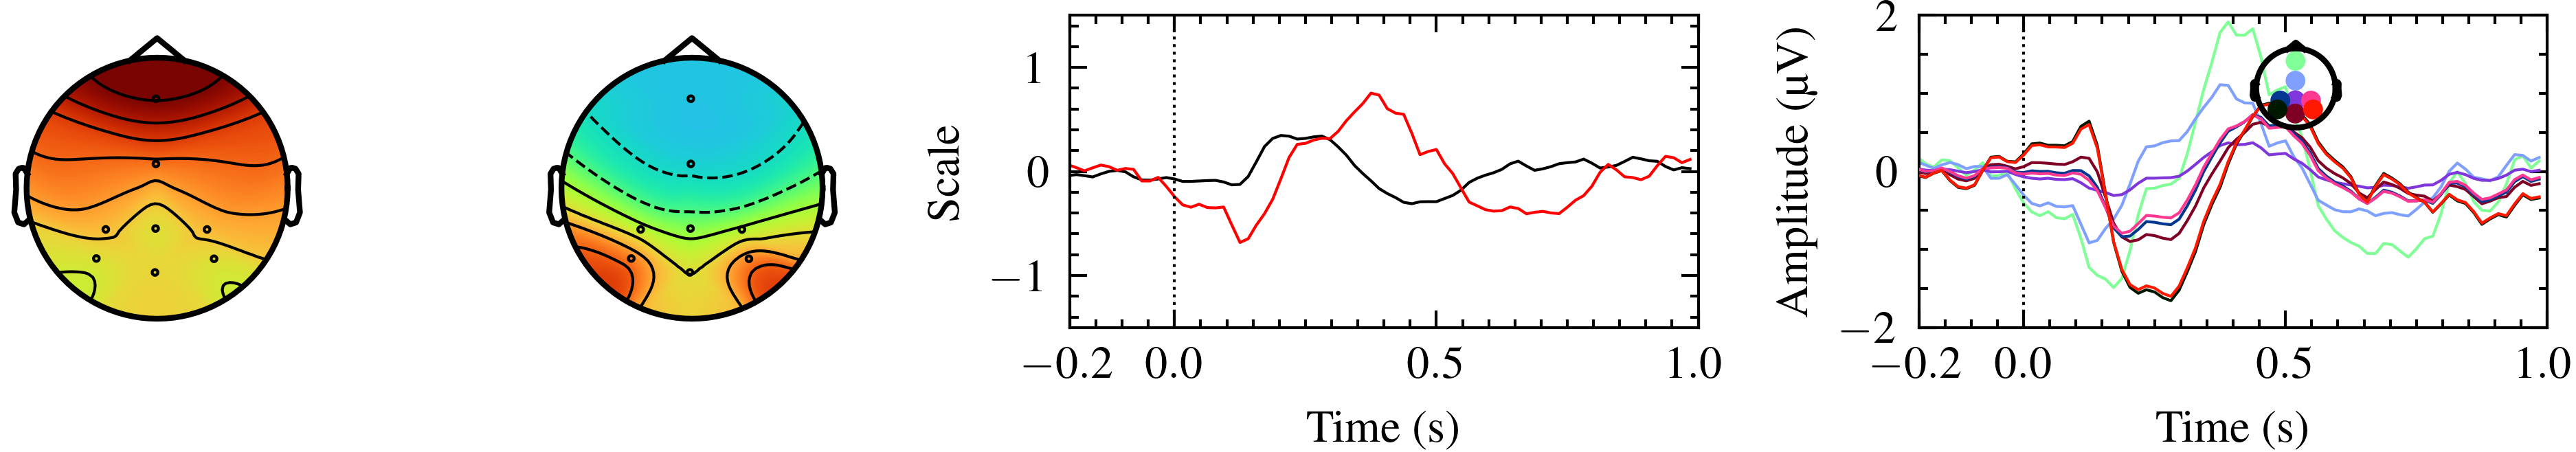
\includegraphics[width=\linewidth]{figure6a.png}
	%	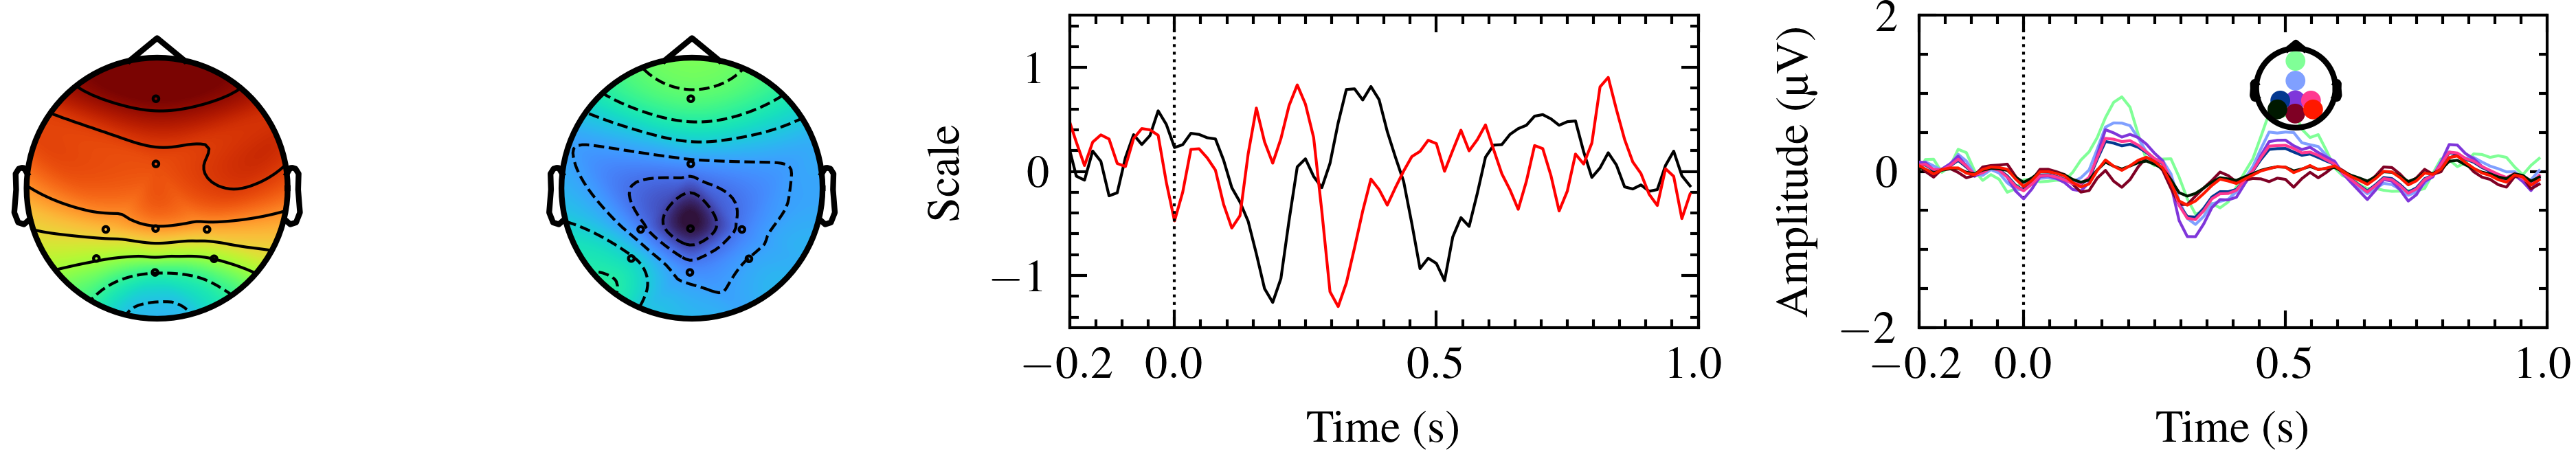
\includegraphics[width=\linewidth]{figure6b.png}
	%  \caption[Extracted \acs{bttda} activation patterns.]{%
	%    Spatial (left two columns) and temporal (middle column) activation patterns and
	%		condition contrasts (right column) obtained after forward projection of the latent
	%    features for 2 blocks of rank $(2,2)$ of \ac{bttda}
	%    fit on the full dataset BNCI2014-008.
	%    The separate blocks approximately model different \ac{erp}
	%		components.}
	%	\label{fig:forward}
	%\end{figure*}
	Given informed or correctly tuned hyperparameters, this method could be used to
	e.g., separate \ac{erp} components or neural processes based on the task-related
	information in the class labels.

	In summary, \ac{bttda} with a proper choice of rank is a useful generalization
	of \ac{hoda}.
	We conclude there is an effective	added value in iteratively finding multiple blocks.
	The flexibility of the \ac{bttda} model is both expressed in its ability
	to capture more discriminant information with more parsimony,
	and in its ability to capture effects such as the covariance structure which
	cannot be expressed by the \ac{hoda} model.
	This makes it suited to tackle classification problems encountered in brain-computer interfacing.

	\subsection{Model selection}

	\Ac{bttda} trades in the rigid \ac{hoda} model for increased model complexity with more
	hyperparameters to tune, which expands the solution space to settings where performance can be
	improved.
	This shifts the focus of tensor discriminant analysis from projection
	optimization to model selection.
	Despite favorable results in \ac{bci} decoding, the applications of the proposed
	\ac{bttda} model are mainly limited by the model selection approach used
	to determine the individual block ranks.
	While our proposed selection procedure controlled by $\theta$
	is a step in the direction of decreasing the computational demand, it
	also limits the chosen ranks of each block to lie within a subset of all possible configurations.
	In a sense, this goes against the earlier proposition of increased model flexibility.
	Instances could occur where \ac{bttda} offers little to no added value over the
	Tucker-structured \ac{hoda} when both are given totally free choice of rank, but cases where \ac{bttda} could achieve greater performance could equally be found.
	Finding these optimal-rank configurations, however, can currently only be achieved
	through a costly, cross-validated hyperparameter search jointly over the ranks of each block.Future efforts should focus on more advanced automated hyperparameter selection methods, e.g., using sparsity,
	eigenvalue truncation, information criteria such as the ones used in
	\ac{bttr}~\cite{Faes2022}, or other statistical measures based on the model's
	application.

	Furthermore, it is clear that our proposed model selection procedure does not
	necessarily result in an optimal set of blocks that group coherent projections
	within the same block according to some desirable metric.
	Currently, features across blocks are heavily correlated, leading to a high
	degree of multicollinearity in the extracted features which we correct for post-hoc
	by applying whitening and PCA.
	Solutions imposing some sense of subspace orthogonality between the extracted blocks
	could lead to a more effective feature extraction solution.
	Other examples of useful within block grouping criteria are sparsity,
	pattern interpretability, minimal or maximal within-block feature correlation,
	ordering of blocks by decreasing discriminability, etc.

	\todo[inline]{This hypothesis seems reasonable, but is not substantiated with
		evidence or analysis, which could feasible be done with some extra work by analyzing the number of features. Is it relevant?}
	A final limitation is that \ac{bttda} might yield a disproportionate
	improvement for datasets with a low number of features relative to sample size,
	while being less effective for datasets with more features.
	This is reflected in our \ac{erp} results (low dimensionality vs.\ high number of
	trials) compared to the \ac{mi} results (higher dimensionality due to third-order
	tensorization vs.\ lower number of trials).
	The impact higher-order tensors with $K>3$ should be thoroughly
	investigated, since this could have a large impact on model behaviour.
	We expect a dimensionality limit beyond which the forward modeling step cannot
	accurately regress from the low-dimensional latent tensors to the high-
	dimensional original tensors, introducing
	error in the input data for the next block which can stack up over blocks.
	Since the forward multilinear least squares problem is underdetermined, it is
	prone to numerical instability, which calls for regularization of the forward
	modeling procedure.
	Unfortunately, using e.g. $L_1$ or $L_2$ regularization would introduce another
hyperparameter.
Finally, other tensorization methods of the \ac{eeg} data, like time-lagged Hankel
tensors~\cite{Papy2005}, or tensors across subjects or sliding windows, etc.,
could also be of interest if they are appropriately chosen based on prior
knowledge of the dataset.

\section{Conclusion}

We have introduced \acf{bttda}, a novel,
tensor-based, supervised dimensionality reduction technique optimized for class
discriminability, which adheres to the block-term tensor structure.
\ac{bttda} is a generalization of \acf{hoda} and can also be
applied as a special sum-of-rank-one tensors \ac{parafacda} model.
The model is obtained by iteratively fitting \ac{hoda} in a deflation scheme,
leveraging a novel forward modeling step.

Via accompanying model selection hyperparameters, \ac{bci} decoders using
\ac{bttda} feature extraction can significantly outperform decoders based on
\ac{hoda} and reach state-of-the-art decoding performance on \acl{erp} problems (second-order tensors) and scores on par with or higher than \ac{hoda} in motor imagery problems (third-order tensors).
Moving from the rigid Tucker tensor structure of \ac{hoda} to the more flexible
and sparse block-term structure shifts the focus from finding the best constrained
multilinear projections to model and feature selection.

This allows performance to be traded off for model complexity and the number of
features, which is particularly relevant for \ac{bci} decoding problems.
Because of its general implementation and minimal assumptions on data structure,
\ac{bttda} can equally be applied to classification for other neuroimaging modalities
(MEG, ECoG, fNIRS, fMRI, EMG, etc.) or to tensor classification problems in other
domains.

\section*{Code availability}

The source code of the proposed \ac{bttda} algorithm and the analyses performed in
this work are available at \url{https://github.com/arnevdk/bttda}.

\section*{Additional data and materials}
\begin{enumerate}
	\item\textbf{Full ERP decoding cross-validation results} \\
	file: \texttt{erp\_results.csv}\\
	format: \textit{comma-separated values file}
	\label{item:add/erp-results}
	\item\textbf{Full MI decoding cross-validation results} \\
	file: \texttt{mi\_results.csv}\\
	format: \textit{comma-separated values file}
	\label{item:add/mi-results}
	\item\textbf{Full results of analysis in function of the number of blocks and block rank}\\
	file: \texttt{block-theta-results.csv}\\
	format: \textit{comma-separated values file}
	\label{item:add/blocks}
\end{enumerate}

\section*{Acknowledgements}
We thank the Flemish Supercomputer Center (VSC) and the High-Performance
Computing (HPC) center of KU Leuven for allowing us to execute our
computational experiments on their systems.
We also wish to acknowledge Dr.\ Axel Faes for his inspiration in
conceptualizing this work.

AVDK is funded by the special research fund of the KU Leuven (GPUDL/20/031).
\todo[inline]{Should past funds used when the work was in preperation also be
	mentioned here, or only those active at the time of submission?}
MMVH is supported by research grants received from the European Union’s
Horizon Europe Marie Sklodowska-Curie Action program
(grant agreement No. 101118964), the European Union’s Horizon 2020 research and
innovation program (grant agreement No. 857375), the special research fund of
the KU Leuven (C24/18/098), the Belgian Fund for Scientific Research – Flanders
(G0A4118N, G0A4321N, G0C1522N), and the Hercules Foundation (AKUL 043).

The authors acknowledge the support of the RITMEA project co-financed by the
European Union with the European Regional Development Fund, the French state,
and the Hauts-de-France Region Council.


\printbibliography%
\clearpage%

\appendix
\setcounter{table}{0}
\renewcommand{\thetable}{A\arabic{table}}

\begin{table*}[ht]
	\footnotesize
	\begin{tabularx}{\linewidth}{@{}Xrrrrrrr@{}}
	\toprule
	Dataset                    & \# Sub.         & \# Chan. & \# Trials/class
	                           & \makecell{Epoch                                                                                          \\ len. (s)} & \makecell{S. freq.\\ (Hz)}
	                           & \# Sess.        & Ref.                                                                                   \\
	\midrule
	\textbf{\Ac{erp} datasets} &                 &          &                 &     &      &                   &                          \\
	BNCI2014-008               & 8               & 8        & 3500/700        & 1.0 & 256  & 1                 & \cite{Riccio2013}        \\
	BNCI2014-009               & 10              & 16       & 1440/288        & 0.8 & 256  & 3                 & \cite{Arico2014}         \\
	BNCI2015-003               & 10              & 8        & 1500/300        & 0.8 & 256  & 1                 & \cite{Guger2009}         \\
	BrainInvaders2012          & 25              & 16       & 640/128         & 1.0 & 128  & 2                 & \cite{VanVeen2019}       \\
	BrainInvaders2013a         & 24              & 16       & 3200/640        & 1.0 & 512  & 8 (sub. 1-7) or 1 & \cite{Vaineau2019}       \\
	BrainInvaders2014a         & 64              & 16       & 990/198         & 1.0 & 512  & up to 3           & \cite{Korczowski2019}    \\
	BrainInvaders2014b         & 38              & 32       & 200/40          & 1.0 & 512  & 3                 & \cite{Korczowski2019a}   \\
	BrainInvaders2015a         & 43              & 32       & 4131/825        & 1.0 & 512  & 3                 & \cite{Korczowski2019b}   \\
	BrainInvaders2015b         & 44              & 32       & 2160/480        & 1.0 & 512  & 1                 & \cite{Korczowski2019c}   \\
	Cattan2019-VR              & 21              & 16       & 600/120         & 1.0 & 512  & 2                 & \cite{Cattan2019}        \\
	%DemonsP300                 & 60              & 8                & 935/50          & 1.0  & 500  & 1                 & \cite{Goncharenko2020}   \\
	EPFLP300                   & 8               & 32       & 2753/551        & 1.0 & 2048 & 4                 & \cite{Hoffmann2008}      \\
	%ErpCore2021-ERN            & 40              & 30               & 400/400         & 1.0  & 1024 & 1                 & \cite{Kappenman2021}     \\
	%ErpCore2021-LRP            & 40              & 30               & 400/400         & 1.0  & 1024 & 1                 & \cite{Kappenman2021}     \\
	%ErpCore2021-MMN            & 40              & 30               & 800/200         & 1.0  & 1024 & 1                 & \cite{Kappenman2021}     \\
	%ErpCore2021-N170           & 40              & 30               & 240/80          & 1.0  & 1024 & 1                 & \cite{Kappenman2021}     \\
	%ErpCore2021-N2pc           & 40              & 30               & 160/160         & 1.0  & 1024 & 1                 & \cite{Kappenman2021}     \\
	%ErpCore2021-N400           & 40              & 30               & 60/60           & 1.0  & 1024 & 1                 & \cite{Kappenman2021}     \\
	%ErpCore2021-P3             & 40              & 30               & 160/40          & 1.0  & 1024 & 1                 & \cite{Kappenman2021}     \\
	Huebner2017                & 13              & 31       & 364/112         & 0.9 & 1000 & 3                 & \cite{Huebner2017}       \\
	Huebner2018                & 12              & 31       & 364/112         & 0.9 & 1000 & 3                 & \cite{Huebner2018}       \\
	Lee2019-ERP                & 54              & 62       & 6900/1380       & 1.0 & 1000 & 2                 & \cite{Lee2019}           \\
	Sosulski2019               & 13              & 31       & 7500/1500       & 1.2 & 1000 & 1                 & \cite{Sosulski2019}      \\
	\midrule
	\textbf{\Ac{mi} datasets}  &                 &          &                 &     &      &                   &                          \\
	AlexandreMotorImagery      & 8               & 16       & 20.0            & 3.0 & 512  & 1                 & \cite{Barachant2012}     \\
	%Beetl2021-A                & 4               & 63               &                 & 4.0  & 500  & 1                 & \cite{Wei2022}           \\
	%Beetl2021-B                & 2               & 32               &                 & 4.0  & 200  & 1                 & \cite{Wei2022}           \\
	BNCI2014-001               & 9               & 22       & 144.0           & 4.0 & 250  & 2                 & \cite{Tangermann2012}    \\
	%BNCI2014-002               & 14              & 15               & 80.0            & 5.0  & 512  & 1                 & \cite{Steyrl2016}        \\
	%BNCI2014-004               & 9               & 3                & 360.0           & 4.5  & 250  & 5                 & \cite{Leeb2007}          \\
	%BNCI2015-001               & 12              & 13               & 200.0           & 5.0  & 512  & 3                 & \cite{Faller2012}        \\
	%BNCI2015-004               & 9               & 30               & 80.0            & 7.0  & 256  & 2                 & \cite{Scherer2015}       \\
	%Cho2017                    & 52              & 64               & 100.0           & 3.0  & 512  & 1                 & \cite{Cho2017}           \\
	%Dreyer2023                 & 87              & 27               & 20.0            & 5.0  & 512  & 1                 & \cite{Pillette2021}      \\
	%Dreyer2023A                & 60              & 27               & 20.0            & 5.0  & 512  & 1                 & \cite{Pillette2021}      \\
	%Dreyer2023B                & 21              & 27               & 20.0            & 5.0  & 512  & 1                 & \cite{Pillette2021}      \\
	%Dreyer2023C                & 6               & 27               & 20.0            & 5.0  & 512  & 1                 & \cite{Pillette2021}      \\
	%GrosseWentrup2009          & 10              & 128              & 150.0           & 7.0  & 500  & 1                 & \cite{GrosseWentrup2009} \\
	%Lee2019-MI                 & 54              & 62               & 100.0           & 4.0  & 1000 & 2                 & \cite{Lee2019}           \\
	%Liu2024                    & 50              & 29               & 20.0            & 4.0  & 500  & 1                 & \cite{Liu2024}           \\
	%Ofner2017                  & 15              & 61               & 60.0            & 3.0  & 512  & 1                 & \cite{Ofner2017}         \\
	%	PhysionetMotorImagery      & 109             & 64       & 23.0            & 3.0 & 160  & 1                 & \cite{Goldberger2000}    \\
	Schirrmeister2017          & 14              & 128      & 120.0           & 4.0 & 500  & 1                 & \cite{Schirrmeister2017} \\
	%Shin2017A                  & 29              & 30               & 30.0            & 10.0 & 200  & 3                 & \cite{Shin2016}          \\
	%Shin2017B                  & 29              & 30               & 30.0            & 10.0 & 200  & 3                 & \cite{Shin2016}          \\
	%Stieger2021                & 62              & 64               & 450.0           & 3.0  & 1000 & 7 or 11           & \cite{Stieger2021}       \\
	Weibo2014                  & 10              & 60       & 80.0            & 4.0 & 200  & 1                 & \cite{Yi2014}            \\
	Zhou2016                   & 4               & 14       & 160.0           & 5.0 & 250  & 3                 & \cite{Zhou2016}          \\
	\bottomrule
\end{tabularx}

	\caption{MOABB datasets used for evaluation, with the number of
		subjects (\# Sub.), the number of EEG channels (\# Chan.), the number of trials or trials per class for ERP
		datasets (\# Trials), the epoch length (Epoch len.), the sampling
		frequency (S. freq.), the number of sessions per subject (\# Sess.) and the
		number of runs (\# Runs). \ac{erp} datasets contain 2 classes, for \ac{mi} datasets the first 3 classes were retained. \Ac{erp} dataset Sosulski2019 was omitted due to technical problems.
		\Ac{mi} dataset PhysionetMI was omitted due to its high computational and
		storage demands.
		Adapted from~\cite{Aristimunha2023}
		and~\cite{Chevallier2024}.}
	\label{tab:moabb}
\end{table*}

\begin{table*}[ht]
	\footnotesize
	\begin{tabular}{@{}lrrrrrr@{}}
\toprule
decoder 1 & \multicolumn{4}{c}{BTTDA} & \multicolumn{2}{c}{PARAFACDA} \\
decoder 2 & \multicolumn{2}{c}{HODA} & \multicolumn{2}{c}{PARAFACDA} & \multicolumn{2}{c}{HODA} \\
 & $p$ & SMD & $p$ & SMD & $p$ & SMD \\
\midrule
BNCI2014-008 & \num{7.81e-03} & 1.43 & \num{8.59e-02} & 0.53 & \num{7.81e-03} & 1.21 \\
BNCI2014-009 & \num{2.25e-02} & 0.75 & \num{6.54e-02} & 0.54 & \num{3.71e-02} & 0.66 \\
BNCI2015-003 & \num{2.93e-03} & 1.32 & \num{8.79e-03} & 0.90 & \num{6.84e-03} & 1.10 \\
BrainInvaders2012 & \num{6.14e-06} & 1.56 & \num{1.33e-01} & 0.28 & \num{7.85e-06} & 1.41 \\
BrainInvaders2013a & \num{4.02e-05} & 1.03 & \num{3.26e-03} & 0.70 & \num{8.77e-05} & 0.87 \\
BrainInvaders2014a & \num{2.06e-11} & 1.17 & \num{4.15e-03} & 0.33 & \num{8.07e-11} & 1.08 \\
BrainInvaders2014b & \num{1.60e-04} & 0.69 & \num{2.39e-02} & 0.35 & \num{2.24e-03} & 0.51 \\
BrainInvaders2015a & \num{3.41e-13} & 1.24 & \num{3.22e-07} & 0.87 & \num{2.21e-08} & 0.93 \\
BrainInvaders2015b & \num{1.88e-12} & 1.43 & \num{2.74e-02} & 0.35 & \num{4.94e-10} & 1.20 \\
Cattan2019-VR & \num{2.62e-05} & 1.16 & \num{2.12e-01} & 0.26 & \num{1.57e-05} & 1.17 \\
EPFLP300 & \num{3.91e-03} & 1.86 & \num{1.56e-02} & 0.93 & \num{1.17e-02} & 1.34 \\
Huebner2017 & \num{1.22e-04} & 0.63 & \num{9.28e-02} & 0.39 & \num{3.66e-04} & 0.62 \\
Huebner2018 & \num{9.77e-04} & 1.16 & \num{3.91e-03} & 0.94 & \num{3.66e-03} & 1.09 \\
Lee2019-ERP & \num{2.10e-09} & 0.88 & \num{1.14e-02} & 0.26 & \num{1.02e-10} & 1.02 \\
\bottomrule
\end{tabular}

	\caption{Results of one-sided Wilcoxon rank-sum tests comparing the
		per-subject cross-validated classification scores of the evaluated \ac{erp}
		decoders.
		Significance is reported as $p$, the effect size as the standardized mean
		difference (SMD).}
	\label{tab:results/erp/stats}
\end{table*}

\begin{table*}[ht]
	\footnotesize
	\begin{tabular}{@{}lrrrrrr@{}}
\toprule
decoder 1 & \multicolumn{4}{c}{BTTDA} & \multicolumn{2}{c}{PARAFACDA} \\
decoder 2 & \multicolumn{2}{c}{HODA} & \multicolumn{2}{c}{PARAFACDA} & \multicolumn{2}{c}{HODA} \\
 & $p$ & SMD & $p$ & SMD & $p$ & SMD \\
\midrule
BNCI2014-008 & \num{3.91e-03} & 1.57 & \num{1.95e-02} & 0.90 & \num{7.81e-03} & 1.31 \\
BNCI2014-009 & \num{5.86e-03} & 0.94 & \num{1.76e-02} & 0.80 & \num{5.47e-02} & 0.58 \\
BNCI2015-003 & \num{2.93e-03} & 1.31 & \num{7.81e-03} & 0.96 & \num{6.84e-03} & 1.11 \\
BrainInvaders2012 & \num{6.14e-06} & 1.74 & \num{1.98e-02} & 0.49 & \num{7.85e-06} & 1.45 \\
BrainInvaders2013a & \num{3.28e-06} & 1.05 & \num{8.00e-02} & 0.22 & \num{1.51e-05} & 0.98 \\
BrainInvaders2014a & \num{2.56e-11} & 1.18 & \num{2.81e-03} & 0.40 & \num{5.71e-11} & 1.14 \\
BrainInvaders2014b & \num{3.02e-04} & 0.62 & \num{1.34e-01} & 0.15 & \num{3.02e-04} & 0.59 \\
BrainInvaders2015a & \num{1.59e-12} & 1.17 & \num{3.22e-07} & 0.84 & \num{8.62e-10} & 1.00 \\
BrainInvaders2015b & \num{2.11e-11} & 1.33 & \num{4.37e-02} & 0.27 & \num{6.47e-10} & 1.19 \\
Cattan2019-VR & \num{6.68e-06} & 1.28 & \num{3.97e-01} & 0.21 & \num{2.38e-06} & 1.38 \\
EPFLP300 & \num{3.91e-03} & 1.72 & \num{3.52e-02} & 0.81 & \num{3.91e-03} & 1.36 \\
Huebner2017 & \num{3.66e-04} & 0.62 & \num{1.37e-01} & 0.32 & \num{4.88e-04} & 0.61 \\
Huebner2018 & \num{1.22e-03} & 1.15 & \num{3.91e-03} & 0.88 & \num{3.17e-03} & 1.10 \\
Lee2019-ERP & \num{8.13e-11} & 1.06 & \num{3.30e-03} & 0.38 & \num{1.08e-10} & 1.02 \\
\bottomrule
\end{tabular}

	\caption{Results of one-sided Wilcoxon rank-sum tests comparing the
		per-subject cross-validated classification scores of the evaluated \ac{mi}
		decoders.
		Significance is reported as $p$, the effect size as the standardized mean
		difference (SMD).}
	\label{tab:results/mi/stats}
\end{table*}

\pagebreak

\end{document}
